%  LaTeX support: latex@mdpi.com
%  For support, please attach all files needed for compiling as well as the log file, and specify your operating system, LaTeX version, and LaTeX editor.

%=================================================================
% pandoc conditionals added to preserve backwards compatibility with previous versions of rticles

\documentclass[notspecified,article,submit,moreauthors,pdftex]{Definitions/mdpi}


%% Some pieces required from the pandoc template
\setlist[itemize]{leftmargin=*,labelsep=5.8mm}
\setlist[enumerate]{leftmargin=*,labelsep=4.9mm}


%--------------------
% Class Options:
%--------------------

%---------
% article
%---------
% The default type of manuscript is "article", but can be replaced by:
% abstract, addendum, article, book, bookreview, briefreport, casereport, comment, commentary, communication, conferenceproceedings, correction, conferencereport, entry, expressionofconcern, extendedabstract, datadescriptor, editorial, essay, erratum, hypothesis, interestingimage, obituary, opinion, projectreport, reply, retraction, review, perspective, protocol, shortnote, studyprotocol, systematicreview, supfile, technicalnote, viewpoint, guidelines, registeredreport, tutorial
% supfile = supplementary materials

%----------
% submit
%----------
% The class option "submit" will be changed to "accept" by the Editorial Office when the paper is accepted. This will only make changes to the frontpage (e.g., the logo of the journal will get visible), the headings, and the copyright information. Also, line numbering will be removed. Journal info and pagination for accepted papers will also be assigned by the Editorial Office.

%------------------
% moreauthors
%------------------
% If there is only one author the class option oneauthor should be used. Otherwise use the class option moreauthors.

%---------
% pdftex
%---------
% The option pdftex is for use with pdfLaTeX. Remove "pdftex" for (1) compiling with LaTeX & dvi2pdf (if eps figures are used) or for (2) compiling with XeLaTeX.

%=================================================================
% MDPI internal commands - do not modify
\firstpage{1}
\makeatletter
\setcounter{page}{\@firstpage}
\makeatother
\pubvolume{1}
\issuenum{1}
\articlenumber{0}
\pubyear{2023}
\copyrightyear{2023}
%\externaleditor{Academic Editor: Firstname Lastname}
\datereceived{ }
\daterevised{ } % Comment out if no revised date
\dateaccepted{ }
\datepublished{ }
%\datecorrected{} % For corrected papers: "Corrected: XXX" date in the original paper.
%\dateretracted{} % For corrected papers: "Retracted: XXX" date in the original paper.
\hreflink{https://doi.org/} % If needed use \linebreak
%\doinum{}
%\pdfoutput=1 % Uncommented for upload to arXiv.org

%=================================================================
% Add packages and commands here. The following packages are loaded in our class file: fontenc, inputenc, calc, indentfirst, fancyhdr, graphicx, epstopdf, lastpage, ifthen, float, amsmath, amssymb, lineno, setspace, enumitem, mathpazo, booktabs, titlesec, etoolbox, tabto, xcolor, colortbl, soul, multirow, microtype, tikz, totcount, changepage, attrib, upgreek, array, tabularx, pbox, ragged2e, tocloft, marginnote, marginfix, enotez, amsthm, natbib, hyperref, cleveref, scrextend, url, geometry, newfloat, caption, draftwatermark, seqsplit
% cleveref: load \crefname definitions after \begin{document}

%=================================================================
% Please use the following mathematics environments: Theorem, Lemma, Corollary, Proposition, Characterization, Property, Problem, Example, ExamplesandDefinitions, Hypothesis, Remark, Definition, Notation, Assumption
%% For proofs, please use the proof environment (the amsthm package is loaded by the MDPI class).

%=================================================================
% Full title of the paper (Capitalized)
\Title{ProyectoAED2023}

% MDPI internal command: Title for citation in the left column
\TitleCitation{ProyectoAED2023}

% Author Orchid ID: enter ID or remove command
%\newcommand{\orcidauthorA}{0000-0000-0000-000X} % Add \orcidA{} behind the author's name
%\newcommand{\orcidauthorB}{0000-0000-0000-000X} % Add \orcidB{} behind the author's name


% Authors, for the paper (add full first names)
\Author{Carlos$^{}$, Diego$^{}$, Miguel$^{}$}


%\longauthorlist{yes}


% MDPI internal command: Authors, for metadata in PDF
\AuthorNames{Carlos, Diego, Miguel}

% MDPI internal command: Authors, for citation in the left column

% Affiliations / Addresses (Add [1] after \address if there is only one affiliation.)
\address{%
$^{1}$ \quad Universidad de Valencia - ETSE, UV Avinguda de
l'Universitat, 46100 Burjassot,
Valencia; \href{mailto:leutnant@fh-muenster.de}{\nolinkurl{leutnant@fh-muenster.de}}\\
$^{2}$ \quad ; \\
}

% Contact information of the corresponding author
\corres{Correspondence: }

% Current address and/or shared authorship








% The commands \thirdnote{} till \eighthnote{} are available for further notes

% Simple summary
\simplesumm{A Simple summary goes here.}

%\conference{} % An extended version of a conference paper

% Abstract (Do not insert blank lines, i.e. \\)
\abstract{Análisis exploratorio de un conjunto de datos sobre la calidad
del aire de la ciudad de Valencia entre 2004 y 2022}


% Keywords
\keyword{Contaminación, Valencia, datos, análisis}

% The fields PACS, MSC, and JEL may be left empty or commented out if not applicable
%\PACS{J0101}
%\MSC{}
%\JEL{}

%%%%%%%%%%%%%%%%%%%%%%%%%%%%%%%%%%%%%%%%%%
% Only for the journal Diversity
%\LSID{\url{http://}}

%%%%%%%%%%%%%%%%%%%%%%%%%%%%%%%%%%%%%%%%%%
% Only for the journal Applied Sciences

%%%%%%%%%%%%%%%%%%%%%%%%%%%%%%%%%%%%%%%%%%

%%%%%%%%%%%%%%%%%%%%%%%%%%%%%%%%%%%%%%%%%%
% Only for the journal Data



%%%%%%%%%%%%%%%%%%%%%%%%%%%%%%%%%%%%%%%%%%
% Only for the journal Toxins


%%%%%%%%%%%%%%%%%%%%%%%%%%%%%%%%%%%%%%%%%%
% Only for the journal Encyclopedia


%%%%%%%%%%%%%%%%%%%%%%%%%%%%%%%%%%%%%%%%%%
% Only for the journal Advances in Respiratory Medicine
%\addhighlights{yes}
%\renewcommand{\addhighlights}{%

%\noindent This is an obligatory section in “Advances in Respiratory Medicine”, whose goal is to increase the discoverability and readability of the article via search engines and other scholars. Highlights should not be a copy of the abstract, but a simple text allowing the reader to quickly and simplified find out what the article is about and what can be cited from it. Each of these parts should be devoted up to 2~bullet points.\vspace{3pt}\\
%\textbf{What are the main findings?}
% \begin{itemize}[labelsep=2.5mm,topsep=-3pt]
% \item First bullet.
% \item Second bullet.
% \end{itemize}\vspace{3pt}
%\textbf{What is the implication of the main finding?}
% \begin{itemize}[labelsep=2.5mm,topsep=-3pt]
% \item First bullet.
% \item Second bullet.
% \end{itemize}
%}


%%%%%%%%%%%%%%%%%%%%%%%%%%%%%%%%%%%%%%%%%%

% Pandoc syntax highlighting
\usepackage{color}
\usepackage{fancyvrb}
\newcommand{\VerbBar}{|}
\newcommand{\VERB}{\Verb[commandchars=\\\{\}]}
\DefineVerbatimEnvironment{Highlighting}{Verbatim}{commandchars=\\\{\}}
% Add ',fontsize=\small' for more characters per line
\usepackage{framed}
\definecolor{shadecolor}{RGB}{248,248,248}
\newenvironment{Shaded}{\begin{snugshade}}{\end{snugshade}}
\newcommand{\AlertTok}[1]{\textcolor[rgb]{0.94,0.16,0.16}{#1}}
\newcommand{\AnnotationTok}[1]{\textcolor[rgb]{0.56,0.35,0.01}{\textbf{\textit{#1}}}}
\newcommand{\AttributeTok}[1]{\textcolor[rgb]{0.13,0.29,0.53}{#1}}
\newcommand{\BaseNTok}[1]{\textcolor[rgb]{0.00,0.00,0.81}{#1}}
\newcommand{\BuiltInTok}[1]{#1}
\newcommand{\CharTok}[1]{\textcolor[rgb]{0.31,0.60,0.02}{#1}}
\newcommand{\CommentTok}[1]{\textcolor[rgb]{0.56,0.35,0.01}{\textit{#1}}}
\newcommand{\CommentVarTok}[1]{\textcolor[rgb]{0.56,0.35,0.01}{\textbf{\textit{#1}}}}
\newcommand{\ConstantTok}[1]{\textcolor[rgb]{0.56,0.35,0.01}{#1}}
\newcommand{\ControlFlowTok}[1]{\textcolor[rgb]{0.13,0.29,0.53}{\textbf{#1}}}
\newcommand{\DataTypeTok}[1]{\textcolor[rgb]{0.13,0.29,0.53}{#1}}
\newcommand{\DecValTok}[1]{\textcolor[rgb]{0.00,0.00,0.81}{#1}}
\newcommand{\DocumentationTok}[1]{\textcolor[rgb]{0.56,0.35,0.01}{\textbf{\textit{#1}}}}
\newcommand{\ErrorTok}[1]{\textcolor[rgb]{0.64,0.00,0.00}{\textbf{#1}}}
\newcommand{\ExtensionTok}[1]{#1}
\newcommand{\FloatTok}[1]{\textcolor[rgb]{0.00,0.00,0.81}{#1}}
\newcommand{\FunctionTok}[1]{\textcolor[rgb]{0.13,0.29,0.53}{\textbf{#1}}}
\newcommand{\ImportTok}[1]{#1}
\newcommand{\InformationTok}[1]{\textcolor[rgb]{0.56,0.35,0.01}{\textbf{\textit{#1}}}}
\newcommand{\KeywordTok}[1]{\textcolor[rgb]{0.13,0.29,0.53}{\textbf{#1}}}
\newcommand{\NormalTok}[1]{#1}
\newcommand{\OperatorTok}[1]{\textcolor[rgb]{0.81,0.36,0.00}{\textbf{#1}}}
\newcommand{\OtherTok}[1]{\textcolor[rgb]{0.56,0.35,0.01}{#1}}
\newcommand{\PreprocessorTok}[1]{\textcolor[rgb]{0.56,0.35,0.01}{\textit{#1}}}
\newcommand{\RegionMarkerTok}[1]{#1}
\newcommand{\SpecialCharTok}[1]{\textcolor[rgb]{0.81,0.36,0.00}{\textbf{#1}}}
\newcommand{\SpecialStringTok}[1]{\textcolor[rgb]{0.31,0.60,0.02}{#1}}
\newcommand{\StringTok}[1]{\textcolor[rgb]{0.31,0.60,0.02}{#1}}
\newcommand{\VariableTok}[1]{\textcolor[rgb]{0.00,0.00,0.00}{#1}}
\newcommand{\VerbatimStringTok}[1]{\textcolor[rgb]{0.31,0.60,0.02}{#1}}
\newcommand{\WarningTok}[1]{\textcolor[rgb]{0.56,0.35,0.01}{\textbf{\textit{#1}}}}

% tightlist command for lists without linebreak
\providecommand{\tightlist}{%
  \setlength{\itemsep}{0pt}\setlength{\parskip}{0pt}}



\usepackage{longtable}

\begin{document}



%%%%%%%%%%%%%%%%%%%%%%%%%%%%%%%%%%%%%%%%%%

\hypertarget{introducciuxf3n}{%
\section{Introducción}\label{introducciuxf3n}}

En el presente informe planteamos el análisis exploratorio de un
conjunto de datos sobre la calidad del aire de la ciudad de Valencia
entre 2004 y 2022. El dataset empleado continene observaciones obtenidas
de distintas estaciones de la red de vigilancia de Valencia. Las
observaciones están compuestas por variables respectivas a diversas
moleculas y elementos presentes en el aire junto a otras de tipo
meteorológico como la velocidad del viento, la temperatura, etc.

El procedimiento a seguir comenzará con la correcta importación del
dataset, a lo que seguirá la preparación de los datos para resolver las
preguntas planteadas. Se escogerán las variables de interés y los
periodos temporales sobre los que se realizará el análisis, se aplicarán
las transformaciones necesarias sobre las variables, se reestructurará
el dataset acorde a nuestras necesidades y se gestionarán los outliers y
datos faltantes.

Una vez preparado el dataset, procederemos a responder a las preguntas
planteadas mediante diversas metodologías. Todo el proceso irá
acompañado de las explicaciones pertinentes y finalizaremos con una
conclusión del trabajo realizado.

\hypertarget{objetivos}{%
\subsection{Objetivos}\label{objetivos}}

El objetivo principal de este trabajo es familizarse con las
herramientas y metodologías aprendidas para la carga, manipulación y
análisis exploratorio de un conjunto de datos.

\begin{itemize}
\tightlist
\item
  analisis univariante, bivariante, NA, outliers
\end{itemize}

Para ello se van a plantear una serie de objetivos es forma de preguntas
que requerirán la aplicación de las herramientas y metodologías
aprendidas:

\begin{itemize}
\item
  ¿?Influencia del cambio en el tráfico hacia el centro de la ciudad en
  los últimos años. (carriles bici) : Comprobar posible reducción de
  gases emitidos por vehículos a motor en las estaciones más céntricas.
\item
  ¿?Existe alguna correlación entre la calidad del aire y el día de la
  semana/año
\item
  ¿?Existe cierta evolución de la contaminación sonora (años/zonas)
\item
  ¿?Existe cierta evolución de la temperatura (A medias, se puede hacer
  algo más o incluso relacionarlo con las precipitaciones. No se me
  ocurre cómo pero se le podría dar una vuelta)
\item
  ¿?Existe cierta evolución de la contaminación. Como medir la
  contaminación (Falta esta)
\end{itemize}

A lo largo del desarrollo del proyecto se irán planteando y resolviendo
las preguntas anteriores junto a su razonamiento y conclusiones.

\hypertarget{carga-de-libreruxedas-y-datos}{%
\subsection{Carga de librerías y
datos}\label{carga-de-libreruxedas-y-datos}}

\begin{Shaded}
\begin{Highlighting}[]
\NormalTok{pacman}\SpecialCharTok{::}\FunctionTok{p\_load}\NormalTok{(readr, lubridate, tidyr, dplyr, ggplot2, plotly, stats)}
\end{Highlighting}
\end{Shaded}

El primer paso es importar nuestro dataset. Para ello, en primer lugar
abrimos (por ejemplo en un bloc de notas) el archivo \emph{rvvcca.csv}
localizado en la carpeta data. De esta forma vemos el formato en el que
están guardados los datos, lo cuál es importante para su correcta
importación. Por ejemplo, vemos que el separador de las variables es
`;', lo cuál debe ser especificado en la función \emph{read\_delim()} de
readr que usamos para la importación. Tembién definimos el formato con
el que queremos importar ciertas columnas, como pueden ser las columnas
de tipo fecha o algunos factores.

\begin{Shaded}
\begin{Highlighting}[]
\CommentTok{\# Especificamos el tipo de columna para que los datos se importen directamente con un formato adecuado}
\NormalTok{column\_types }\OtherTok{\textless{}{-}} \FunctionTok{cols}\NormalTok{(}
  \AttributeTok{Fecha =} \FunctionTok{col\_date}\NormalTok{(}\AttributeTok{format =} \StringTok{"\%Y{-}\%m{-}\%d"}\NormalTok{),}
  \StringTok{\textasciigrave{}}\AttributeTok{Dia de la semana}\StringTok{\textasciigrave{}} \OtherTok{=} \FunctionTok{col\_factor}\NormalTok{(}\AttributeTok{levels =} \FunctionTok{c}\NormalTok{(}\StringTok{"Lunes"}\NormalTok{, }\StringTok{"Martes"}\NormalTok{,  }\StringTok{"Miercoles"}\NormalTok{, }\StringTok{"Jueves"}\NormalTok{, }\StringTok{"Viernes"}\NormalTok{, }\StringTok{"Sabado"}\NormalTok{, }\StringTok{"Domingo"}\NormalTok{)),}
  \StringTok{\textasciigrave{}}\AttributeTok{Dia del mes}\StringTok{\textasciigrave{}} \OtherTok{=} \FunctionTok{col\_factor}\NormalTok{(}\AttributeTok{levels =} \FunctionTok{as.character}\NormalTok{(}\DecValTok{1}\SpecialCharTok{:}\DecValTok{31}\NormalTok{)),}
  \AttributeTok{Estacion =} \FunctionTok{col\_factor}\NormalTok{(),}
  \StringTok{\textasciigrave{}}\AttributeTok{Fecha creacion}\StringTok{\textasciigrave{}}\OtherTok{=} \FunctionTok{col\_date}\NormalTok{(}\AttributeTok{format =} \StringTok{"\%Y{-}\%m{-}\%d"}\NormalTok{),}
  \StringTok{\textasciigrave{}}\AttributeTok{Fecha baja}\StringTok{\textasciigrave{}}\OtherTok{=} \FunctionTok{col\_date}\NormalTok{(}\AttributeTok{format =} \StringTok{"\%Y{-}\%m{-}\%d"}\NormalTok{))}

\CommentTok{\# importación del dataset}
\NormalTok{datos }\OtherTok{\textless{}{-}} \FunctionTok{read\_delim}\NormalTok{(}\StringTok{"data/rvvcca.csv"}\NormalTok{, }\AttributeTok{delim =} \StringTok{";"}\NormalTok{, }\AttributeTok{escape\_double =} \ConstantTok{FALSE}\NormalTok{, }\AttributeTok{trim\_ws =} \ConstantTok{TRUE}\NormalTok{, }\AttributeTok{col\_types =}\NormalTok{ column\_types)}
\FunctionTok{head}\NormalTok{(datos)}
\end{Highlighting}
\end{Shaded}

\begin{verbatim}
## # A tibble: 6 x 34
##      Id Fecha      `Dia de la semana` `Dia del mes` Estacion     PM1 PM2.5  PM10
##   <dbl> <date>     <fct>              <fct>         <fct>      <dbl> <dbl> <dbl>
## 1     5 2004-03-01 Sabado             3             Pista Sil~    NA    NA  NA  
## 2     7 2004-04-01 Domingo            4             Pista Sil~    NA    NA  NA  
## 3     8 2004-04-01 Domingo            4             Viveros       NA    NA  27.8
## 4     9 2004-05-01 Lunes              5             Pista Sil~    NA    NA  NA  
## 5    14 2004-07-01 Miercoles          7             Viveros       NA    NA  43.9
## 6    26 2004-01-13 Martes             13            Viveros       NA    NA  33.8
## # i 26 more variables: NO <dbl>, NO2 <dbl>, NOx <dbl>, O3 <dbl>, SO2 <dbl>,
## #   CO <dbl>, NH3 <dbl>, C7H8 <dbl>, C6H6 <dbl>, Ruido <dbl>, C8H10 <dbl>,
## #   `Velocidad del viento` <dbl>, `Direccion del viento` <dbl>,
## #   Temperatura <dbl>, `Humidad relativa` <dbl>, Presion <dbl>,
## #   `Radiacion solar` <dbl>, Precipitacion <dbl>,
## #   `Velocidad maxima del viento` <dbl>, `As (ng/m³)` <dbl>,
## #   `Ni (ng/m³)` <dbl>, `Cd (ng/m³)` <dbl>, `Pb (ng/m³)` <dbl>, ...
\end{verbatim}

Para evitar posibles problemas, renombramos las varianles con espacios
en su nombre para trabajar sin comillas ' ' y eliminamos el sufijo
(ng/m³) que aparece en algunas variables

\begin{Shaded}
\begin{Highlighting}[]
\FunctionTok{colnames}\NormalTok{(datos) }\OtherTok{\textless{}{-}} \FunctionTok{gsub}\NormalTok{(}\AttributeTok{x =} \FunctionTok{colnames}\NormalTok{(datos), }\AttributeTok{pattern=}\StringTok{\textquotesingle{} \textquotesingle{}}\NormalTok{, }\AttributeTok{replacement =} \StringTok{\textquotesingle{}\_\textquotesingle{}}\NormalTok{)}
\FunctionTok{colnames}\NormalTok{(datos) }\OtherTok{\textless{}{-}} \FunctionTok{gsub}\NormalTok{(}\AttributeTok{x =} \FunctionTok{colnames}\NormalTok{(datos), }\AttributeTok{pattern=}\StringTok{\textquotesingle{}\_[(]ng[/]m³[)]$\textquotesingle{}}\NormalTok{, }\AttributeTok{replacement =} \StringTok{\textquotesingle{}\textquotesingle{}}\NormalTok{)}
\end{Highlighting}
\end{Shaded}

Para observar las características generales de nuestro dataset vamos a
resumir en una tabla el tipo de cada variable \emph{tyoe}, cuantos
valores distintos tiene \emph{levels}, su valor más frecuente
\emph{topLevel}, cuántas veces aparece \emph{topCount}, y en qué
proporción \emph{topFreq} y por último la proporción de datos faltantes
de cada variable \emph{missFreq}:

\begin{Shaded}
\begin{Highlighting}[]
\NormalTok{levels }\OtherTok{\textless{}{-}} \ControlFlowTok{function}\NormalTok{(x)\{}
  \FunctionTok{as.character}\NormalTok{(}\FunctionTok{length}\NormalTok{(}\FunctionTok{unique}\NormalTok{(x)))}
\NormalTok{\}}

\NormalTok{topLevel }\OtherTok{\textless{}{-}} \ControlFlowTok{function}\NormalTok{(x)\{}
  \FunctionTok{names}\NormalTok{(}\FunctionTok{which.max}\NormalTok{(}\FunctionTok{table}\NormalTok{(x)))}
\NormalTok{\}}

\NormalTok{topCount }\OtherTok{\textless{}{-}} \ControlFlowTok{function}\NormalTok{(x)\{}
  \FunctionTok{as.character}\NormalTok{(}\FunctionTok{sum}\NormalTok{(}\FunctionTok{as.character}\NormalTok{(x)}\SpecialCharTok{==}\FunctionTok{names}\NormalTok{(}\FunctionTok{which.max}\NormalTok{(}\FunctionTok{table}\NormalTok{(x))), }\AttributeTok{na.rm =}\NormalTok{ T))}
\NormalTok{\}}

\NormalTok{topFrec }\OtherTok{\textless{}{-}} \ControlFlowTok{function}\NormalTok{(x)\{}
  \FunctionTok{as.character}\NormalTok{(}\FunctionTok{round}\NormalTok{(}\FunctionTok{sum}\NormalTok{(}\FunctionTok{as.character}\NormalTok{(x)}\SpecialCharTok{==}\FunctionTok{names}\NormalTok{(}\FunctionTok{which.max}\NormalTok{(}\FunctionTok{table}\NormalTok{(x))), }\AttributeTok{na.rm =}\NormalTok{ T)}\SpecialCharTok{/}\FunctionTok{length}\NormalTok{(x), }\AttributeTok{digits =} \DecValTok{3}\NormalTok{))}
\NormalTok{\}}

\NormalTok{missFrec }\OtherTok{\textless{}{-}} \ControlFlowTok{function}\NormalTok{(x)\{}
  \FunctionTok{as.character}\NormalTok{(}\FunctionTok{round}\NormalTok{(}\FunctionTok{sum}\NormalTok{(}\FunctionTok{is.na}\NormalTok{(x))}\SpecialCharTok{/}\FunctionTok{length}\NormalTok{(x), }\AttributeTok{digits=}\DecValTok{3}\NormalTok{))}
\NormalTok{\}}

\NormalTok{sumario }\OtherTok{\textless{}{-}} \FunctionTok{list}\NormalTok{(}\AttributeTok{type =} \SpecialCharTok{\textasciitilde{}}\FunctionTok{class}\NormalTok{(.x), }\AttributeTok{levels =} \SpecialCharTok{\textasciitilde{}}\FunctionTok{levels}\NormalTok{(.x), }\AttributeTok{topLevel =} \SpecialCharTok{\textasciitilde{}}\FunctionTok{topLevel}\NormalTok{(.x), }\AttributeTok{topCount =} \SpecialCharTok{\textasciitilde{}}\FunctionTok{topCount}\NormalTok{(.x), }\AttributeTok{topFrec =} \SpecialCharTok{\textasciitilde{}}\FunctionTok{topFrec}\NormalTok{(.x), }\AttributeTok{missFrec =} \SpecialCharTok{\textasciitilde{}}\FunctionTok{missFrec}\NormalTok{(.x))}

\NormalTok{datos }\SpecialCharTok{\%\textgreater{}\%}
  \FunctionTok{summarise}\NormalTok{(}\FunctionTok{across}\NormalTok{(}\AttributeTok{.cols =} \FunctionTok{all\_of}\NormalTok{(}\FunctionTok{colnames}\NormalTok{(datos)), }\AttributeTok{.fns =}\NormalTok{ sumario, }\AttributeTok{.names =} \StringTok{"\{.col\}{-}\{.fn\}"}\NormalTok{)) }\SpecialCharTok{\%\textgreater{}\%} 
  \FunctionTok{pivot\_longer}\NormalTok{(}\AttributeTok{cols =} \DecValTok{1}\SpecialCharTok{:}\DecValTok{203}\NormalTok{, }\AttributeTok{names\_to =} \StringTok{\textquotesingle{}variable\_estadistica\textquotesingle{}}\NormalTok{, }\AttributeTok{values\_to =} \StringTok{\textquotesingle{}valor\textquotesingle{}}\NormalTok{) }\SpecialCharTok{\%\textgreater{}\%}
  \FunctionTok{separate}\NormalTok{(variable\_estadistica, }\AttributeTok{into =}  \FunctionTok{c}\NormalTok{(}\StringTok{\textquotesingle{}variable\textquotesingle{}}\NormalTok{, }\StringTok{\textquotesingle{}estadistica\textquotesingle{}}\NormalTok{), }\AttributeTok{sep =} \StringTok{\textquotesingle{}{-}\textquotesingle{}}\NormalTok{) }\SpecialCharTok{\%\textgreater{}\%}
  \FunctionTok{pivot\_wider}\NormalTok{(}\AttributeTok{names\_from =} \StringTok{\textquotesingle{}estadistica\textquotesingle{}}\NormalTok{, }\AttributeTok{values\_from =} \StringTok{\textquotesingle{}valor\textquotesingle{}}\NormalTok{)}
\end{Highlighting}
\end{Shaded}

\begin{verbatim}
## # A tibble: 34 x 7
##    variable         type    levels topLevel    topCount topFrec missFrec
##    <chr>            <chr>   <chr>  <chr>       <chr>    <chr>   <chr>   
##  1 Id               numeric 43388  1           1        0       0       
##  2 Fecha            Date    6940   2022-01-01  12       0       0       
##  3 Dia_de_la_semana factor  7      Sabado      6205     0.143   0       
##  4 Dia_del_mes      factor  31     16          1426     0.033   0       
##  5 Estacion         factor  13     Pista Silla 6940     0.16    0       
##  6 PM1              numeric 179    4           978      0.023   0.748   
##  7 PM2.5            numeric 221    9           1567     0.036   0.463   
##  8 PM10             numeric 479    13          1104     0.025   0.336   
##  9 NO               numeric 178    2           3890     0.09    0.23    
## 10 NO2              numeric 120    16          961      0.022   0.23    
## # i 24 more rows
\end{verbatim}

\begin{itemize}
\item
  \emph{Id} es un identificador para cada una de las filas y no aporta
  ninguna información concreta.
\item
  \emph{Fecha} es una variable tipo \emph{Date} que nos proporciona la
  fecha en la que se tomaron los datos que componen la observación.
  Tomaremos esta variable para la ordenación ascendente de los datos.
  Vemos que hay datos de casi 7000 días distintos y que el día con más
  datos (esto se corresponde a más estaciones distintas midiendo 12/13)
  es el 01-01-2022.
\end{itemize}

\begin{Shaded}
\begin{Highlighting}[]
\NormalTok{datos }\OtherTok{\textless{}{-}} \FunctionTok{arrange}\NormalTok{(datos,datos}\SpecialCharTok{$}\NormalTok{Fecha)}
\end{Highlighting}
\end{Shaded}

\begin{itemize}
\item
  \emph{Dia\_de\_la\_semana} y \emph{Dia\_del\_mes} son variables de
  tipo factor que indican en que día de la semana y en qué día del mes
  se realiza la medida. Puede ser extraído a partir de \emph{Fecha}
  usando las funciones \emph{wday()} y \emph{day()}, de la librería
  \emph{lubridate}. Vemos que el día de la semana más repetido es el
  Sábado y el del mes es el 31, sin embargo sus frecuecnias son
  prácticamente 1/7 y 1/30 por lo que parece indicar que todos los días
  de la semana y del mes están en la misma proporción. Esto estaría
  enconcordancia con el hecho de que tenemos datos realmente diarios.
\item
  \emph{Estacion} es una variable de tipo factor cuyos niveles son las
  distintas estaciones meteorológicas donde se tomaron las mediciones de
  las variables numéricas, haciendo un total de 13 estaciones. La más
  repetida es la estación de Pista de Silla con una frecuencia de 0.16
  \textgreater{} 1/13 = 0.077. Esto significa que es la estación que
  aparece en más días distintos, y es indicativo de que no todas las
  estaciones funcionan durante el mismo tiempo.
\end{itemize}

\begin{Shaded}
\begin{Highlighting}[]
\FunctionTok{unique}\NormalTok{(datos}\SpecialCharTok{$}\NormalTok{Estacion)}
\end{Highlighting}
\end{Shaded}

\begin{verbatim}
##  [1] Pista Silla               Viveros                  
##  [3] Politecnico               Avda. Francia            
##  [5] Moli del Sol              Bulevard Sud             
##  [7] Conselleria Meteo         Puerto Valencia          
##  [9] Valencia Centro           Nazaret Meteo            
## [11] Puerto llit antic Turia   Puerto Moll Trans. Ponent
## [13] Valencia Olivereta       
## 13 Levels: Pista Silla Viveros Politecnico Avda. Francia ... Puerto Valencia
\end{verbatim}

\begin{itemize}
\item
  \emph{PM1, PM2.5, PM10} son variables de tipo numérico con datos sobre
  la concentración de materiales particuldos (PM) de menos de 1, 2.5 y
  10 micrómetros de diámetro respectivamente. Pese a ser variables
  numéricas supuestamente continuas llama a la atención que no hay un
  gran número de niveles distintos comparado con el número de filas del
  del dataset (alrededor de 10 veces menos). También vemos que hay un
  gran número de datos faltantes, sobre todo para PM1 (más de un 70\%) y
  esto puede explicar en parte que no haya tantos valores distintos. Sin
  embargo, también podría deberse a que quizá durante muchos días el
  nivel de concentración de esas partículas se mantiene constante (o al
  menos la sensibilidad del sensor que las mide no es capaz de medir tal
  diferencia). La gran cantidad de datos faltantes puede deberse a que
  las varaibles no se miden durante ciertos períodos de tiempo o en
  todas las estaciones.
\item
  \emph{NO, NO2, NOx, O2, SO2, CO, NH3} son variables con datos sobre la
  concentración de estas moléculas inorgánicas consideradas
  contaminantes en el aire. Respecto a los óxidos de nitrógeno (NOx),
  estos son un grupo de gases compuestos por oxígeno y nitrógeno, es
  decir, NO y NO2 forman parte de este grupo y por lo tanto los valores
  de las variables estarán altamente correlacionados. La proporción de
  NA's en estas variables menor en este caso, alrededor del 20\% con
  excepción del NH3 que presenta más de un 90\% de datos faltantes. De
  nuevo el número de NA's puede deberse a los mismos motivos
  argumentados anteriormente y que comprobaremos más adelante en el
  análisis. Por otro lado, también tenemos unos pocos cientos de valores
  distintos para ser también variables numéricas continuas y esto puede
  deberse a las mismas causas argumentadas para los materiales
  particulados.
\item
  \emph{C7H8, C6H6, C8H10} son variables con datos sobre la
  concentración de estas moléculas orgánicas también consideradas
  contaminantes en el aire. De nuevo estas variables numéricas y
  continuas presentan datos faltantes por encima del 90\% y muchos menos
  niveles distintos que observacioness de las variables. Podrían
  ofrecerse los mismos argumentos para explicar estos hechos. El
  porcentaje similar de datos faltantes podría se debido a que estas
  variables se miden al vez (en las mismas estaciones y períodos de
  tiempo).
\item
  \emph{Velocidad\_del\_viento, Direccion\_del\_viento, Temperatura,
  Humidad\_relativa, Presion, Radiacion\_solar, Precipitacion,
  Velocidad\_maxima\_del\_viento} son variables numéricas con mediciones
  de estas distintas condiciones ambientales al momento de medir las
  concentraciones de moléculas contaminantes en el aire. Es interesante
  contar con estos datos para ver si influyen en los valores de
  contaminación. Estas variables presentan entre un 50-60\% de datos
  faltantes que puede deberse a que no todas las estacione miden las
  condiciones ambientales.
\item
  \emph{As, Ni, Cd, Pb} son variables numéricas con datos de otras
  concentraciones de gases y metales contaminantes en el aire. Todos
  estas variables presentaban el prefijo (ng/m3) indicando las unidades
  en que se mide sus concentraciones. El resto de datos de
  concentraciones no presentan las unidades lo cuál nos hace sospechar
  que auiás los datos de estas variables fueron medidas en conjunto.
  Esto también explicaría que todos tengan el mismo porcentaje de datos
  faltantes (entorno al 98\%). De nuevo, en el análisis comprobaremos a
  qué puede deberse esta cantidad de datos faltantes.
\item
  \emph{B(a)p} es una variable booleana que sólo presenta una
  observación. Elresto de datos son faltants y no podemos saber lo que
  representa esta variable.
\item
  \emph{Fecha\_creación} y \emph{Fecha\_baja} son variables de tipo
  \emph{Date} que parecen estar relacionadas con la creacion del dataset
  y que no parecen aportar información sobre nuestros datos.
  \emph{Fecha\_creación} solo presenta dos entradas distintas y
  \emph{Fecha\_baja} sólo presenta NA's por lo que estas variables
  parecen prescindibles.
\end{itemize}

Vamos a mantener sólo las variables que aporten alguna información
relevante:

\begin{Shaded}
\begin{Highlighting}[]
\NormalTok{datos }\OtherTok{\textless{}{-}}\NormalTok{ datos }\SpecialCharTok{\%\textgreater{}\%} \FunctionTok{select}\NormalTok{(}\SpecialCharTok{{-}}\FunctionTok{c}\NormalTok{(}\StringTok{\textquotesingle{}Id\textquotesingle{}}\NormalTok{, }\StringTok{\textquotesingle{}Dia\_de\_la\_semana\textquotesingle{}}\NormalTok{,}\StringTok{\textquotesingle{}Dia\_del\_mes\textquotesingle{}}\NormalTok{,}\StringTok{\textquotesingle{}Fecha\_creacion\textquotesingle{}}\NormalTok{, }\StringTok{\textquotesingle{}Fecha\_baja\textquotesingle{}}\NormalTok{, }\StringTok{\textquotesingle{}B(a)p\textquotesingle{}}\NormalTok{))}
\end{Highlighting}
\end{Shaded}

\hypertarget{anuxe1lisis-de-datos-faltantes-y-especiales}{%
\section{Análisis de datos faltantes y
especiales}\label{anuxe1lisis-de-datos-faltantes-y-especiales}}

En esta sección, previamente al análisis univariante y bivariante de las
variables, vamos a realizar un análisis de la estructura del dataset. El
dataset parece estar compuesto por la unión de un conjunto datasets,
posiblemente por las distintas estaciones de las que provienen los
datos. Con el objetivo de obtener un conjunto de datos consistente,
analizaremos el porcentaje de NA's que hay por cada variable, luego
veremos que datos proporcionan las estaciones y con que frecuencia,
también comprobaremos cuando comenzaron a generar datos las estaciones y
durante que periodos de tiempo se han obtenido las variables.

En primer lugar vamos reemplazar todos los posibles valores especiales
(NULL, NaN, Inf\ldots) que pudieran haber en las varianles numéricas de
nuestro dataset por NA's. De esta forma podemos tratar todos estos datos
que no tienen sentido a la vez.

\begin{Shaded}
\begin{Highlighting}[]
\NormalTok{variables\_numericas }\OtherTok{\textless{}{-}} \FunctionTok{colnames}\NormalTok{(datos[}\FunctionTok{sapply}\NormalTok{(datos,is.numeric)])}
\NormalTok{reemplazo\_especiales }\OtherTok{\textless{}{-}} \ControlFlowTok{function}\NormalTok{(x)\{}
  \FunctionTok{return}\NormalTok{(}\FunctionTok{ifelse}\NormalTok{(}\FunctionTok{is.finite}\NormalTok{(x), x, }\ConstantTok{NA}\NormalTok{))}
\NormalTok{\}}
\NormalTok{datos }\OtherTok{\textless{}{-}} \FunctionTok{mutate}\NormalTok{(datos, }\FunctionTok{across}\NormalTok{(}\FunctionTok{all\_of}\NormalTok{(variables\_numericas), reemplazo\_especiales))}
\end{Highlighting}
\end{Shaded}

Ya hemos visto que nuestras variables numéricas tienen un alto
porcentaje de NA's:

\begin{Shaded}
\begin{Highlighting}[]
\NormalTok{porc\_na }\OtherTok{\textless{}{-}} \ControlFlowTok{function}\NormalTok{(x)\{}
  \DecValTok{100}\SpecialCharTok{*}\FunctionTok{sum}\NormalTok{(}\FunctionTok{is.na}\NormalTok{(x))}\SpecialCharTok{/}\FunctionTok{length}\NormalTok{(x)}
\NormalTok{\}}
\NormalTok{datos }\SpecialCharTok{\%\textgreater{}\%} 
  \FunctionTok{summarise}\NormalTok{(}\FunctionTok{across}\NormalTok{(}\AttributeTok{.cols =} \FunctionTok{all\_of}\NormalTok{(}\FunctionTok{colnames}\NormalTok{(datos)), }\AttributeTok{.fns =}\NormalTok{ porc\_na)) }\SpecialCharTok{\%\textgreater{}\%} 
  \FunctionTok{pivot\_longer}\NormalTok{(}\AttributeTok{cols =} \FunctionTok{all\_of}\NormalTok{(}\FunctionTok{colnames}\NormalTok{(datos)), }\AttributeTok{names\_to =} \StringTok{\textquotesingle{}Variable\textquotesingle{}}\NormalTok{, }\AttributeTok{values\_to =} \StringTok{"Porcentaje NA\textquotesingle{}s"}\NormalTok{) }\SpecialCharTok{\%\textgreater{}\%}
  \FunctionTok{arrange}\NormalTok{(}\FunctionTok{desc}\NormalTok{(}\StringTok{\textasciigrave{}}\AttributeTok{Porcentaje NA\textquotesingle{}s}\StringTok{\textasciigrave{}}\NormalTok{)) }\SpecialCharTok{\%\textgreater{}\%} 
  \FunctionTok{mutate}\NormalTok{(}\StringTok{\textasciigrave{}}\AttributeTok{Porcentaje NA\textquotesingle{}s}\StringTok{\textasciigrave{}}\OtherTok{=}\FunctionTok{round}\NormalTok{(}\StringTok{\textasciigrave{}}\AttributeTok{Porcentaje NA\textquotesingle{}s}\StringTok{\textasciigrave{}}\NormalTok{, }\AttributeTok{digits =} \DecValTok{2}\NormalTok{))}
\end{Highlighting}
\end{Shaded}

\begin{verbatim}
## # A tibble: 28 x 2
##    Variable `Porcentaje NA's`
##    <chr>                <dbl>
##  1 Ni                    97.8
##  2 Pb                    97.8
##  3 As                    97.8
##  4 Cd                    97.8
##  5 NH3                   94.0
##  6 C7H8                  90.8
##  7 C6H6                  90.2
##  8 C8H10                 90.1
##  9 Ruido                 75.1
## 10 PM1                   74.8
## # i 18 more rows
\end{verbatim}

Como ya hemos comentado, pensamos que el elevado número de datos
faltantes puede deberse a que algunas variables se miden en peródos de
tiempo diferentes a las demás o a que no en todas las estaciones se
miden todas las variables. Al unir los datos de las distintas estaciones
por la fecha, se habrían dado lugar los NA's. Para comprobar esta teoría
vamos a realizar una serie de representacions gráficas exploratorias.

En primer lugar, creamos un mapa de calor para comprobar cuáles son las
variables que mide cada estación y cuántos datos de dicha variable
aporta cada estación.

\begin{Shaded}
\begin{Highlighting}[]
\NormalTok{num\_entradas }\OtherTok{\textless{}{-}} \ControlFlowTok{function}\NormalTok{(x)\{}
  \FunctionTok{sum}\NormalTok{(}\SpecialCharTok{!}\FunctionTok{is.na}\NormalTok{(x))}
\NormalTok{\}}
\NormalTok{est\_var }\OtherTok{\textless{}{-}}\NormalTok{ datos }\SpecialCharTok{\%\textgreater{}\%} 
  \FunctionTok{group\_by}\NormalTok{(Estacion) }\SpecialCharTok{\%\textgreater{}\%} 
  \FunctionTok{summarise}\NormalTok{(}\FunctionTok{across}\NormalTok{(}\AttributeTok{.cols =} \FunctionTok{all\_of}\NormalTok{(variables\_numericas), }\AttributeTok{.fns =}\NormalTok{ num\_entradas)) }\SpecialCharTok{\%\textgreater{}\%} 
  \FunctionTok{pivot\_longer}\NormalTok{(}\AttributeTok{cols =} \FunctionTok{all\_of}\NormalTok{(variables\_numericas), }\AttributeTok{names\_to =} \StringTok{\textquotesingle{}Variable\textquotesingle{}}\NormalTok{, }\AttributeTok{values\_to =} \StringTok{"Numero\_entradas"}\NormalTok{) }\SpecialCharTok{\%\textgreater{}\%}
  \FunctionTok{mutate}\NormalTok{(}\AttributeTok{Variable =} \FunctionTok{factor}\NormalTok{(Variable, }\AttributeTok{levels =}\NormalTok{ variables\_numericas, }\AttributeTok{ordered =}\NormalTok{ T)) }\SpecialCharTok{\%\textgreater{}\%} 
  \FunctionTok{arrange}\NormalTok{(}\FunctionTok{match}\NormalTok{(Variable, variables\_numericas))}

\NormalTok{p }\OtherTok{\textless{}{-}} \FunctionTok{ggplot}\NormalTok{(}\AttributeTok{data =}\NormalTok{ est\_var, }\FunctionTok{aes}\NormalTok{(}\AttributeTok{x =}\NormalTok{ Estacion, }\AttributeTok{y=}\NormalTok{Variable, }\AttributeTok{fill =}\NormalTok{ Numero\_entradas)) }\SpecialCharTok{+} 
  \FunctionTok{geom\_tile}\NormalTok{() }\SpecialCharTok{+} \FunctionTok{scale\_fill\_gradient}\NormalTok{(}\AttributeTok{low =} \StringTok{"white"}\NormalTok{, }\AttributeTok{high =} \StringTok{"blue"}\NormalTok{) }\SpecialCharTok{+} 
  \FunctionTok{theme}\NormalTok{(}\AttributeTok{axis.text.x=}\FunctionTok{element\_text}\NormalTok{(}\AttributeTok{angle=}\DecValTok{45}\NormalTok{, }\AttributeTok{hjust=}\DecValTok{1}\NormalTok{))}

\CommentTok{\#plotly::ggplotly(p)}
\end{Highlighting}
\end{Shaded}

En este mapa de calor podemos ver qué variables mide cada estación
meteorológica, además de la cantidad de datos que aporta cada una de
ellas sobre cada varaible numérica. Vemos como sólo hay dos estaciones
(Viveros y Boulevard Sud) que miden las variables \emph{As}, \emph{Pb},
\emph{Ni} y \emph{Cd} y que su número de entradas es bajo en comparación
con otras variable, quizá debido a que se empezaron a tomar datos de
estas variables más tarde que el resto. En el caso del \emph{NH3} vemos
que solo se ha medido en la estación Boulevard Sud. Las moléculas
orgánicas \emph{C8H10}, \emph{C6H6}, \emph{C7H8} sólo se miden en las
estaciones de Pista de Silla y Viveros. Cabe destacar también que las
estaciones que miden mayor cantidad de variables son Pista de Silla,
Viveros y Boulevard Sud. Por otro lado, estaciones como Conselleria
Meteo y Nazaret Meteo sólo miden las condiciones ambientales y no las
concentraciones de contaminantes, al igual que la estación del Puerto de
Valencia con la diferencia que en esta además se miden los niveles de
partículas \emph{PM10} y de \emph{SO2}. Además, vemos como en la
estación de Valencia Olivereta sólo se miden niveles de partículas
\emph{PM2.5}, \emph{PM10} y óxidos de nitrógeno.

Ahora queremos ver qué estaciones han estado activas a lo largo de los
años:

\begin{Shaded}
\begin{Highlighting}[]
\NormalTok{datos }\SpecialCharTok{\%\textgreater{}\%} 
  \FunctionTok{mutate}\NormalTok{(}\AttributeTok{ano =} \FunctionTok{factor}\NormalTok{(}\FunctionTok{year}\NormalTok{(Fecha))) }\SpecialCharTok{\%\textgreater{}\%} 
  \FunctionTok{ggplot}\NormalTok{(}\FunctionTok{aes}\NormalTok{(}\AttributeTok{x=}\NormalTok{ano, }\AttributeTok{fill =}\NormalTok{ Estacion)) }\SpecialCharTok{+} 
  \FunctionTok{geom\_bar}\NormalTok{() }\SpecialCharTok{+} 
  \FunctionTok{labs}\NormalTok{(}\AttributeTok{x =} \StringTok{\textquotesingle{}Año\textquotesingle{}}\NormalTok{) }\SpecialCharTok{+} 
  \FunctionTok{theme}\NormalTok{(}\AttributeTok{axis.text.x=}\FunctionTok{element\_text}\NormalTok{(}\AttributeTok{angle=}\DecValTok{45}\NormalTok{, }\AttributeTok{hjust=}\DecValTok{1}\NormalTok{))}
\end{Highlighting}
\end{Shaded}

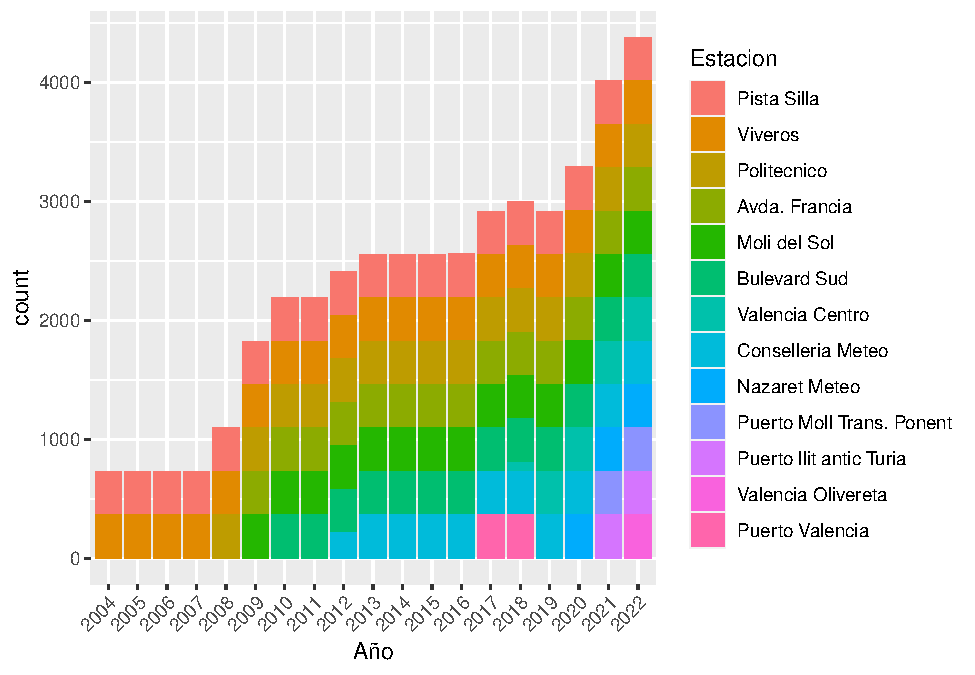
\includegraphics{ProyectoAED2023_plantilla_files/figure-latex/unnamed-chunk-11-1.pdf}

Como podemos ver, desde 2004 hasta 2007 sólo tenemos datos de las
estaciones de Pista de Silla y Viveros, que se mantienen actvas hasta
2022. Posteriormente, en los siguientes 5 años (2008-2012) se van
añadiendo datos de otras estaciones como la del Politécnico, Av. de
Francia, Molí del Sol, Boulevard Sur, Valencia Centro y Conselleria a
razón casi de una nueva estación al año y que se mantienen hasta el
final (2022). Desde 2013 hasta 2016 se siguen viendo las mismas
estaciones y en los siguientes dos años (2017-2018) se añaden datos de
la estación del Puerto de Valencia, de la que posteriormente dejamos de
obtener datos. Finalmente, desde 2019 hasta 2022 se van añadiendo
progresivamente cada año las estaciones de Nazaret, Puerto Molí Trans.
Ponent, Puerto antic Turia y Valencia Olivereta. 2022 es el año donde
tenemos datos de más estaciones distintas.

A continuación queremos visualizar el período de tiempo entre la primera
y la última medida de cada variable

\begin{Shaded}
\begin{Highlighting}[]
\NormalTok{datos }\SpecialCharTok{\%\textgreater{}\%} 
  \FunctionTok{pivot\_longer}\NormalTok{(}\AttributeTok{cols =} \FunctionTok{all\_of}\NormalTok{(variables\_numericas), }\AttributeTok{names\_to =} \StringTok{\textquotesingle{}Variables\textquotesingle{}}\NormalTok{, }\AttributeTok{values\_to =} \StringTok{\textquotesingle{}valor\textquotesingle{}}\NormalTok{, }\AttributeTok{values\_drop\_na =}\NormalTok{ T) }\SpecialCharTok{\%\textgreater{}\%} 
  \FunctionTok{mutate}\NormalTok{(}\AttributeTok{Variables =} \FunctionTok{factor}\NormalTok{(Variables, }\AttributeTok{levels =}\NormalTok{ variables\_numericas, }\AttributeTok{ordered =}\NormalTok{ T)) }\SpecialCharTok{\%\textgreater{}\%} 
  \FunctionTok{ggplot}\NormalTok{(}\FunctionTok{aes}\NormalTok{(}\AttributeTok{x=}\NormalTok{Fecha, }\AttributeTok{y=}\NormalTok{valor, }\AttributeTok{color =}\NormalTok{ Variables)) }\SpecialCharTok{+} 
  \FunctionTok{geom\_line}\NormalTok{() }\SpecialCharTok{+} 
  \FunctionTok{facet\_wrap}\NormalTok{(Variables}\SpecialCharTok{\textasciitilde{}}\NormalTok{., }\AttributeTok{scales =} \StringTok{"free\_y"}\NormalTok{) }\SpecialCharTok{+} 
  \FunctionTok{theme}\NormalTok{(}\AttributeTok{legend.position =} \StringTok{"none"}\NormalTok{) }\SpecialCharTok{+} 
  \FunctionTok{theme}\NormalTok{(}\AttributeTok{axis.text.x=}\FunctionTok{element\_text}\NormalTok{(}\AttributeTok{angle=}\DecValTok{45}\NormalTok{, }\AttributeTok{hjust=}\DecValTok{1}\NormalTok{), }\AttributeTok{axis.text.y =} \FunctionTok{element\_blank}\NormalTok{(), }\AttributeTok{axis.ticks.y =} \FunctionTok{element\_blank}\NormalTok{()) }\SpecialCharTok{+} 
  \FunctionTok{labs}\NormalTok{(}\AttributeTok{y =} \StringTok{\textquotesingle{}\textquotesingle{}}\NormalTok{) }\SpecialCharTok{+} 
  \FunctionTok{scale\_colour\_manual}\NormalTok{(}\AttributeTok{values =} \FunctionTok{rainbow}\NormalTok{(}\DecValTok{26}\NormalTok{)) }
\end{Highlighting}
\end{Shaded}

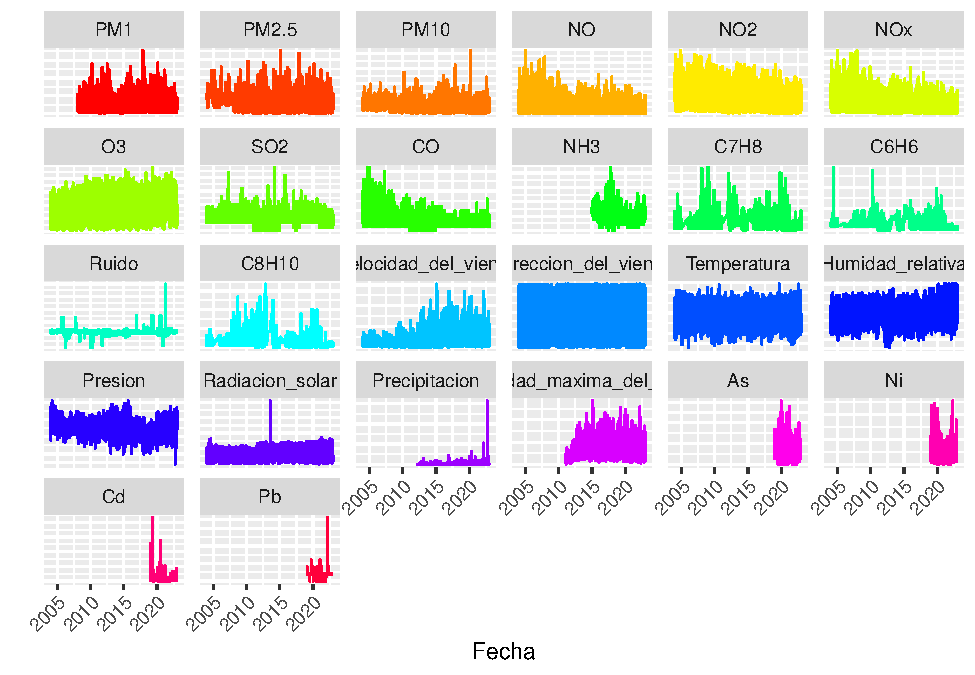
\includegraphics{ProyectoAED2023_plantilla_files/figure-latex/unnamed-chunk-12-1.pdf}

A partir de este gráfico podemos ver como algunas variables empiezan a
ser medidas a partir de cierta fecha. En concreto, los datos de
\emph{As}, \emph{Cd}, \emph{Ni}, \emph{Pb} empiezan a tomarse sólo a
partir de 2019. Además, terminan antes que el resto de variables, a
principios del 2022.. Otras variables como \emph{Precipitacion},
\emph{Velocidad\_maxima\_del\_viento},\emph{PM1} o \emph{NH3} empiezan a
tener datos un poco más tarde que el resto pero antes del 2019. Todas
las demás variables presentan almenos algún dato en 2004.

Tras esta primera visualización de nuestros datos, podemos concluir que
la gran cantidad de datos faltantes se debe a una combinación del hecho
de que no todas las estaciones miden todas las variables, sumado a que
los datos de ciertas variables se empiezan a medir posteriormente que el
resto. Esto puede deberse a que la(s) estación(es) que recoge(n) datos
de esta variable comienza(n) a funcionar en una fecha posterior al resto
de estaciones o simplemente debido a que hasta cierto año no se instalan
sensores en las estaciones para medir esas variables. En cualquier caso,
dependiendo del análisis que se quiera realizar se habrán de escoger
unas variables, y por ende un determinado número de estaciones que midan
estas variables y un período de tiempo en que se estén recogiendo datos
de estas variables.

En nuestro caso vamos a escoger un período de 10 años, desde 2012 a
2022, ya que en este período de tiempo hay un número significativo de
estaciones recogiendo datos y la mayoría de las variables son medidas en
este intervalo de tiempo de forma consistente. No obstante, decidimos
descartar las variables \emph{Pb}, \emph{Cd}, \emph{Ni}, \emph{As},
\emph{B(a)p} y \emph{NH3} debido a que se comienzan a medir después del
2012 y resultaría poco razonable imputar los datos de estas variables en
esos años. De la misma forma, también descartamos las variables
\emph{C7H8}, \emph{C6H6}, y \emph{C8H10} debido a que presentan grandes
períodos de tiempo con ausencia de datos intercalados entre 2012 y 2022,
por lo que también sería poco razonable imputar estos datos.

\hypertarget{anuxe1lisis-univariante}{%
\section{Análisis univariante}\label{anuxe1lisis-univariante}}

En esta sección analizaremos las variables de forma individual con el
objetivo de conocer sus magnitudes, es decir, las unidades de medida que
representan, y como se distribuyen. Como se ha mencionado previamente,
escogemos los datos que comienzan en 2012, concretamente cunado se
empiezan a tomar datos de la precipitación, y los datos previos a 2023,
concretamente cuando se dejan de tomar los oxidos de nitrogeno.

Variables de interés - Fecha - Estación - Gases: NO, NO2, NOx, SO2, CO,
O3 - Meteorológicas: Temperatura, Humedad, Presion, Velocidad viento,
Direccion viento, Radiación solar, Precipitación - Calidad de vida:
Ruido

Comenzamos con un summary de las variables numéricas para analizar las
magnitudes de las variables y como se distribuyen los datos.

\begin{Shaded}
\begin{Highlighting}[]
\NormalTok{variables }\OtherTok{\textless{}{-}} \FunctionTok{c}\NormalTok{(}\StringTok{"Fecha"}\NormalTok{, }\StringTok{"Estacion"}\NormalTok{,}\StringTok{"NO"}\NormalTok{, }\StringTok{"NO2"}\NormalTok{, }\StringTok{"NOx"}\NormalTok{, }\StringTok{"SO2"}\NormalTok{, }\StringTok{"CO"}\NormalTok{, }\StringTok{"O3"}\NormalTok{, }\StringTok{"Temperatura"}\NormalTok{, }\StringTok{"Velocidad\_del\_viento"}\NormalTok{, }\StringTok{"Direccion\_del\_viento"}\NormalTok{, }\StringTok{"Humidad\_relativa"}\NormalTok{, }\StringTok{"Presion"}\NormalTok{, }\StringTok{"Radiacion\_solar"}\NormalTok{, }\StringTok{"Precipitacion"}\NormalTok{,}\StringTok{"Ruido"}\NormalTok{)}

\NormalTok{mystats }\OtherTok{\textless{}{-}} \ControlFlowTok{function}\NormalTok{(x, }\AttributeTok{na.omit=}\ConstantTok{TRUE}\NormalTok{)\{}
                \ControlFlowTok{if}\NormalTok{ (na.omit)}
\NormalTok{                    x }\OtherTok{\textless{}{-}}\NormalTok{ x[}\SpecialCharTok{!}\FunctionTok{is.na}\NormalTok{(x)]}
\NormalTok{                min }\OtherTok{\textless{}{-}} \FunctionTok{min}\NormalTok{(x)}
\NormalTok{                Q1 }\OtherTok{\textless{}{-}} \FunctionTok{quantile}\NormalTok{(x, }\FloatTok{0.25}\NormalTok{)}
\NormalTok{                median }\OtherTok{\textless{}{-}} \FunctionTok{median}\NormalTok{(x)}
\NormalTok{                mean }\OtherTok{\textless{}{-}} \FunctionTok{mean}\NormalTok{(x)}
\NormalTok{                dt }\OtherTok{\textless{}{-}} \FunctionTok{sd}\NormalTok{(x)}
\NormalTok{                Q3 }\OtherTok{\textless{}{-}} \FunctionTok{quantile}\NormalTok{(x, }\FloatTok{0.75}\NormalTok{)}
\NormalTok{                max }\OtherTok{\textless{}{-}} \FunctionTok{max}\NormalTok{(x)}
                
\NormalTok{                n }\OtherTok{\textless{}{-}} \FunctionTok{length}\NormalTok{(x)}
\NormalTok{                IQR }\OtherTok{\textless{}{-}} \FunctionTok{IQR}\NormalTok{(x)}
                
                \FunctionTok{return}\NormalTok{(}\FunctionTok{round}\NormalTok{(}\FunctionTok{c}\NormalTok{(}\AttributeTok{min=}\NormalTok{min, }\AttributeTok{Q1=}\NormalTok{Q1, }\AttributeTok{median=}\NormalTok{median, }\AttributeTok{mean=}\NormalTok{mean, }\AttributeTok{dt=}\NormalTok{dt, }\AttributeTok{Q3=}\NormalTok{Q3, }\AttributeTok{max=}\NormalTok{max, }\AttributeTok{n=}\NormalTok{n, }\AttributeTok{IQR=}\NormalTok{IQR),}\DecValTok{2}\NormalTok{))}
\NormalTok{\} }

\NormalTok{precipitacion }\OtherTok{\textless{}{-}}\NormalTok{ datos[,}\FunctionTok{c}\NormalTok{(}\StringTok{\textquotesingle{}Fecha\textquotesingle{}}\NormalTok{,}\StringTok{\textquotesingle{}Precipitacion\textquotesingle{}}\NormalTok{)] }\SpecialCharTok{\%\textgreater{}\%}\NormalTok{ na.omit}
\NormalTok{fecha\_inicio }\OtherTok{\textless{}{-}}\NormalTok{ precipitacion}\SpecialCharTok{$}\NormalTok{Fecha[}\DecValTok{1}\NormalTok{]}
\NormalTok{oxidos\_n }\OtherTok{\textless{}{-}}\NormalTok{ datos[,}\FunctionTok{c}\NormalTok{(}\StringTok{\textquotesingle{}Fecha\textquotesingle{}}\NormalTok{,}\StringTok{\textquotesingle{}NOx\textquotesingle{}}\NormalTok{)] }\SpecialCharTok{\%\textgreater{}\%}\NormalTok{ na.omit}
\NormalTok{fecha\_fin }\OtherTok{\textless{}{-}}\NormalTok{ oxidos\_n}\SpecialCharTok{$}\NormalTok{Fecha[}\FunctionTok{nrow}\NormalTok{(oxidos\_n)]}

\NormalTok{datos }\OtherTok{\textless{}{-}}\NormalTok{ datos[datos}\SpecialCharTok{$}\NormalTok{Fecha }\SpecialCharTok{\textgreater{}}\NormalTok{ fecha\_inicio }\SpecialCharTok{\&}\NormalTok{ datos}\SpecialCharTok{$}\NormalTok{Fecha }\SpecialCharTok{\textless{}}\NormalTok{ fecha\_fin, variables]}

\FunctionTok{sapply}\NormalTok{(datos[}\SpecialCharTok{{-}}\FunctionTok{c}\NormalTok{(}\DecValTok{1}\NormalTok{,}\DecValTok{2}\NormalTok{)], mystats)}
\end{Highlighting}
\end{Shaded}

\begin{verbatim}
##              NO      NO2      NOx      SO2       CO       O3 Temperatura
## min        0.00     0.00     0.00     0.00     0.00     3.00        4.40
## Q1.25%     3.00    14.00    18.00     3.00     0.10    38.00       13.90
## median     6.00    22.00    32.00     3.00     0.10    53.00       18.50
## mean      10.83    25.58    41.93     3.40     0.16    50.83       18.86
## dt        13.36    15.42    33.85     1.43     0.09    19.15        5.75
## Q3.75%    13.00    35.00    55.00     4.00     0.20    64.00       24.10
## max      152.00   104.00   331.00    24.00     0.80   122.00       34.20
## n      25107.00 25105.00 25107.00 24064.00 12261.00 23958.00    12950.00
## IQR       10.00    21.00    37.00     1.00     0.10    26.00       10.20
##        Velocidad_del_viento Direccion_del_viento Humidad_relativa  Presion
## min                    0.10                 0.00            14.00   968.00
## Q1.25%                 1.00                67.00            55.00  1002.00
## median                 1.60               220.00            67.00  1007.00
## mean                   2.01               179.31            65.81  1007.73
## dt                     1.56               110.28            14.51     8.56
## Q3.75%                 2.40               274.00            76.00  1014.00
## max                   15.20               360.00           100.00  1042.00
## n                  16261.00             16226.00         12652.00 13037.00
## IQR                    1.40               207.00            21.00    12.00
##        Radiacion_solar Precipitacion   Ruido
## min              -7.00          0.00    6.00
## Q1.25%          126.00          0.00   55.00
## median          200.00          0.00   59.00
## mean            200.75          1.26   58.08
## dt               94.03          8.93    6.77
## Q3.75%          281.00          0.00   61.00
## max            1025.00        629.00  250.00
## n             12841.00      11725.00 5157.00
## IQR             155.00          0.00    6.00
\end{verbatim}

Mediante el summary anterior podemos averiguar cuales son las unidades
de medida empleadas contrastando con información externa, ya que en la
fuente de los datos no se proporcionan.

\begin{itemize}
\tightlist
\item
  Gases (NO, NO2, NOx, SO2, CO, O3): microgramos por metro cubico
  (\(\mu\)g/m3)
\item
  Temperatura: grados centígrados (Cº)
\item
  Humedad: porcentaje (\%)
\item
  Presión: hectopascales (hPa)
\item
  Velocidad del viento: kilometros/hora (m/s)
\item
  Dirección del viento: ángulo de 0 a 360 (º)
\item
  Precipitación: litros de agua por metro cuadrado (mm)
\item
  Radiación solar: Vatios por metro cuadrado (W/m2)
\item
  Ruido: decibelios (dB)
\end{itemize}

Densidades:

\begin{Shaded}
\begin{Highlighting}[]
\CommentTok{\# Gases}
\NormalTok{datos[}\DecValTok{2}\SpecialCharTok{:}\DecValTok{8}\NormalTok{] }\SpecialCharTok{\%\textgreater{}\%}
  \FunctionTok{pivot\_longer}\NormalTok{(}\AttributeTok{cols =} \DecValTok{2}\SpecialCharTok{:}\DecValTok{7}\NormalTok{, }\AttributeTok{names\_to =} \StringTok{\textquotesingle{}Variables\textquotesingle{}}\NormalTok{, }\AttributeTok{values\_to =} \StringTok{\textquotesingle{}valor\textquotesingle{}}\NormalTok{, }\AttributeTok{values\_drop\_na =}\NormalTok{ T) }\SpecialCharTok{\%\textgreater{}\%}
  \FunctionTok{ggplot}\NormalTok{(}\FunctionTok{aes}\NormalTok{(}\AttributeTok{x=}\NormalTok{valor)) }\SpecialCharTok{+} 
  \FunctionTok{geom\_histogram}\NormalTok{(}\FunctionTok{aes}\NormalTok{(}\AttributeTok{y=}\FunctionTok{stat}\NormalTok{(density), }\AttributeTok{fill=}\StringTok{\textquotesingle{}blue\textquotesingle{}}\NormalTok{, }\AttributeTok{alpha=}\FloatTok{0.6}\NormalTok{), }\AttributeTok{bins=}\DecValTok{50}\NormalTok{) }\SpecialCharTok{+}
  \FunctionTok{geom\_density}\NormalTok{() }\SpecialCharTok{+}
  \FunctionTok{facet\_wrap}\NormalTok{(}\SpecialCharTok{\textasciitilde{}}\NormalTok{Variables, }\AttributeTok{scales =} \StringTok{"free"}\NormalTok{) }\SpecialCharTok{+} 
  \FunctionTok{theme}\NormalTok{(}\AttributeTok{legend.position =} \StringTok{"none"}\NormalTok{)}
\end{Highlighting}
\end{Shaded}

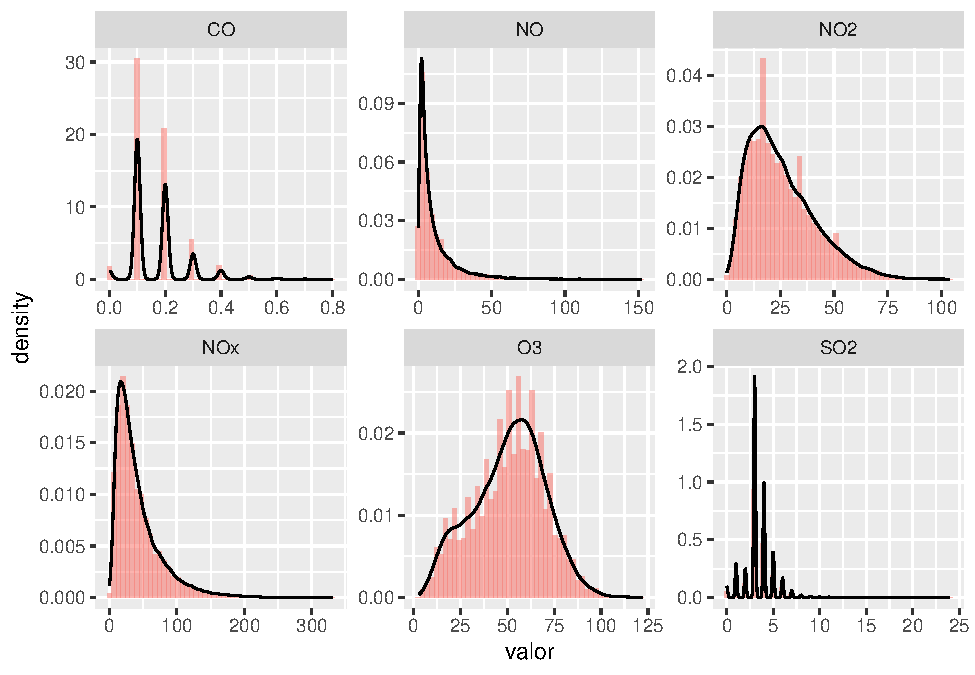
\includegraphics{ProyectoAED2023_plantilla_files/figure-latex/unnamed-chunk-14-1.pdf}

\begin{Shaded}
\begin{Highlighting}[]
\CommentTok{\# Meteorológicas y Ruido}
\NormalTok{datos[}\FunctionTok{c}\NormalTok{(}\DecValTok{2}\NormalTok{,}\FunctionTok{c}\NormalTok{(}\DecValTok{9}\SpecialCharTok{:}\DecValTok{16}\NormalTok{))] }\SpecialCharTok{\%\textgreater{}\%}
  \FunctionTok{pivot\_longer}\NormalTok{(}\AttributeTok{cols =} \DecValTok{2}\SpecialCharTok{:}\DecValTok{9}\NormalTok{, }\AttributeTok{names\_to =} \StringTok{\textquotesingle{}Variables\textquotesingle{}}\NormalTok{, }\AttributeTok{values\_to =} \StringTok{\textquotesingle{}valor\textquotesingle{}}\NormalTok{, }\AttributeTok{values\_drop\_na =}\NormalTok{ T) }\SpecialCharTok{\%\textgreater{}\%}
  \FunctionTok{ggplot}\NormalTok{(}\FunctionTok{aes}\NormalTok{(}\AttributeTok{x=}\NormalTok{valor)) }\SpecialCharTok{+} 
  \FunctionTok{geom\_histogram}\NormalTok{(}\FunctionTok{aes}\NormalTok{(}\AttributeTok{y=}\FunctionTok{stat}\NormalTok{(density), }\AttributeTok{fill=}\StringTok{\textquotesingle{}blue\textquotesingle{}}\NormalTok{, }\AttributeTok{alpha=}\FloatTok{0.6}\NormalTok{), }\AttributeTok{bins=}\DecValTok{50}\NormalTok{) }\SpecialCharTok{+}
  \FunctionTok{geom\_density}\NormalTok{() }\SpecialCharTok{+}
  \FunctionTok{facet\_wrap}\NormalTok{(}\SpecialCharTok{\textasciitilde{}}\NormalTok{Variables, }\AttributeTok{scales =} \StringTok{"free"}\NormalTok{) }\SpecialCharTok{+} 
  \FunctionTok{theme}\NormalTok{(}\AttributeTok{legend.position =} \StringTok{"none"}\NormalTok{)}
\end{Highlighting}
\end{Shaded}

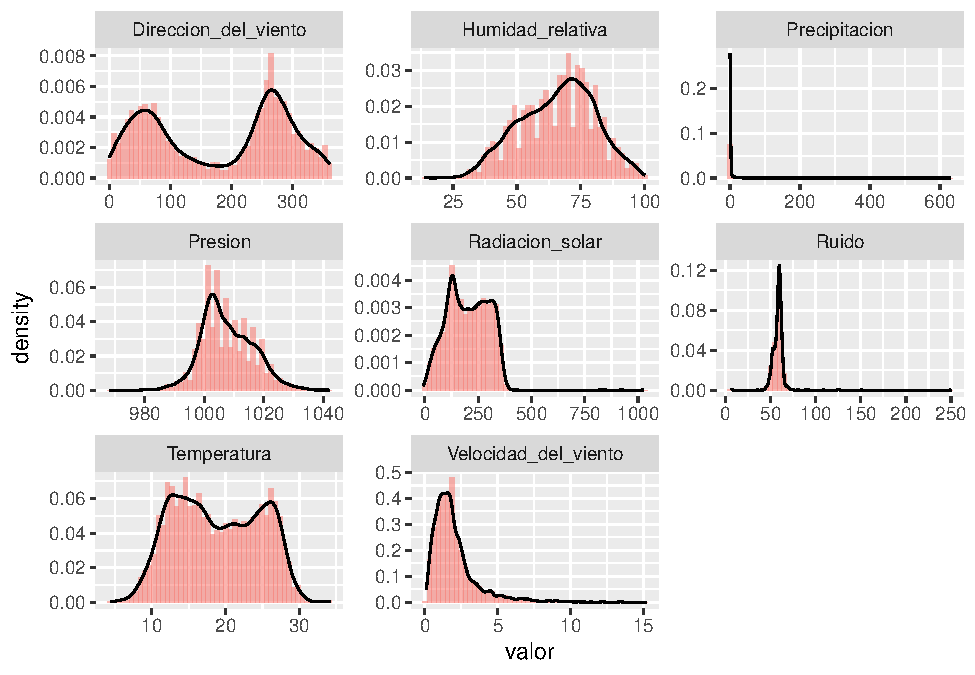
\includegraphics{ProyectoAED2023_plantilla_files/figure-latex/unnamed-chunk-15-1.pdf}

\hypertarget{detecciuxf3n-y-eliminaciuxf3n-de-outliers-con-muxe9todos-univariante}{%
\subsection{Detección y eliminación de outliers con métodos
univariante}\label{detecciuxf3n-y-eliminaciuxf3n-de-outliers-con-muxe9todos-univariante}}

A continuación, procederemos a detectar y eliminar outliers. Primero,
comenzaremos definiendo diferentes funciones posibles para aplicar la
detección de estos. Todas estas funciones corresponden a métodos
univariantes.

\begin{Shaded}
\begin{Highlighting}[]
\NormalTok{tresSigma }\OtherTok{\textless{}{-}} \ControlFlowTok{function}\NormalTok{(x)\{}
\NormalTok{  media }\OtherTok{\textless{}{-}} \FunctionTok{mean}\NormalTok{(x,}\AttributeTok{na.rm=}\ConstantTok{TRUE}\NormalTok{)}
\NormalTok{  desviacion }\OtherTok{\textless{}{-}} \FunctionTok{sd}\NormalTok{(x,}\AttributeTok{na.rm=}\ConstantTok{TRUE}\NormalTok{)}
\NormalTok{  lim\_low }\OtherTok{\textless{}{-}}\NormalTok{ media }\SpecialCharTok{{-}} \DecValTok{3} \SpecialCharTok{*}\NormalTok{ desviacion}
\NormalTok{  lim\_upp }\OtherTok{\textless{}{-}}\NormalTok{ media }\SpecialCharTok{+} \DecValTok{3} \SpecialCharTok{*}\NormalTok{ desviacion}
  
\NormalTok{  outliers }\OtherTok{\textless{}{-}}\NormalTok{ x[x }\SpecialCharTok{\textless{}}\NormalTok{ lim\_low }\SpecialCharTok{|}\NormalTok{ x }\SpecialCharTok{\textgreater{}}\NormalTok{ lim\_upp]}
  
  \FunctionTok{return}\NormalTok{(outliers)}
\NormalTok{\}}

\NormalTok{hampel }\OtherTok{\textless{}{-}} \ControlFlowTok{function}\NormalTok{(x)\{}
\NormalTok{  mediana }\OtherTok{\textless{}{-}} \FunctionTok{median}\NormalTok{(x, }\AttributeTok{na.rm =} \ConstantTok{TRUE}\NormalTok{)}
\NormalTok{  madm }\OtherTok{\textless{}{-}} \FunctionTok{mad}\NormalTok{(x, }\AttributeTok{constant =} \FloatTok{1.4826}\NormalTok{, }\AttributeTok{na.rm =} \ConstantTok{TRUE}\NormalTok{)}
\NormalTok{  umbral }\OtherTok{\textless{}{-}} \DecValTok{3} \SpecialCharTok{*}\NormalTok{ madm}
  
\NormalTok{  outliers }\OtherTok{\textless{}{-}}\NormalTok{ x[}\FunctionTok{abs}\NormalTok{(x}\SpecialCharTok{{-}}\NormalTok{mediana) }\SpecialCharTok{\textgreater{}}\NormalTok{ umbral]}
  
  \FunctionTok{return}\NormalTok{(outliers)}
\NormalTok{\}}

\NormalTok{boxplot }\OtherTok{\textless{}{-}} \ControlFlowTok{function}\NormalTok{(x)\{}
\NormalTok{  q1 }\OtherTok{\textless{}{-}} \FunctionTok{quantile}\NormalTok{(x, }\FloatTok{0.25}\NormalTok{, }\AttributeTok{na.rm =} \ConstantTok{TRUE}\NormalTok{)}
\NormalTok{  q3 }\OtherTok{\textless{}{-}} \FunctionTok{quantile}\NormalTok{(x, }\FloatTok{0.75}\NormalTok{, }\AttributeTok{na.rm =} \ConstantTok{TRUE}\NormalTok{)}
  
\NormalTok{  iqr }\OtherTok{\textless{}{-}}\NormalTok{ q3 }\SpecialCharTok{{-}}\NormalTok{ q1}
  
\NormalTok{  lower\_limit }\OtherTok{\textless{}{-}}\NormalTok{ q1 }\SpecialCharTok{{-}} \FloatTok{1.5} \SpecialCharTok{*}\NormalTok{ iqr}
\NormalTok{  upper\_limit }\OtherTok{\textless{}{-}}\NormalTok{ q3 }\SpecialCharTok{+} \FloatTok{1.5} \SpecialCharTok{*}\NormalTok{ iqr}
  
\NormalTok{  outliers }\OtherTok{\textless{}{-}}\NormalTok{ x[x }\SpecialCharTok{\textless{}}\NormalTok{ lower\_limit }\SpecialCharTok{|}\NormalTok{ x }\SpecialCharTok{\textgreater{}}\NormalTok{ upper\_limit]}
  
  \FunctionTok{return}\NormalTok{(outliers)}
\NormalTok{\}}

\NormalTok{percentil }\OtherTok{\textless{}{-}} \ControlFlowTok{function}\NormalTok{(x)\{}
\NormalTok{  p5 }\OtherTok{\textless{}{-}} \FunctionTok{quantile}\NormalTok{(x, }\FloatTok{0.05}\NormalTok{, }\AttributeTok{na.rm =} \ConstantTok{TRUE}\NormalTok{)}
\NormalTok{  p95 }\OtherTok{\textless{}{-}} \FunctionTok{quantile}\NormalTok{(x, }\FloatTok{0.95}\NormalTok{, }\AttributeTok{na.rm =} \ConstantTok{TRUE}\NormalTok{)}
  
\NormalTok{  outliers }\OtherTok{\textless{}{-}}\NormalTok{ x[x }\SpecialCharTok{\textless{}}\NormalTok{ p5 }\SpecialCharTok{|}\NormalTok{ x }\SpecialCharTok{\textgreater{}}\NormalTok{ p95]}
  
  \FunctionTok{return}\NormalTok{(outliers)}
\NormalTok{\}}

\NormalTok{remove\_outliers }\OtherTok{\textless{}{-}} \ControlFlowTok{function}\NormalTok{(x, func) \{}
\NormalTok{  outliers }\OtherTok{\textless{}{-}} \FunctionTok{func}\NormalTok{(x)}
  \FunctionTok{return}\NormalTok{(x[}\SpecialCharTok{!}\FunctionTok{is.na}\NormalTok{(outliers)])}
\NormalTok{\}}

\NormalTok{replace\_outliers }\OtherTok{\textless{}{-}} \ControlFlowTok{function}\NormalTok{(x, func) \{}
\NormalTok{  outliers }\OtherTok{\textless{}{-}} \FunctionTok{func}\NormalTok{(x)}
\NormalTok{  x[outliers] }\OtherTok{\textless{}{-}} \ConstantTok{NA}
  \FunctionTok{return}\NormalTok{(x)}
\NormalTok{\}}
\end{Highlighting}
\end{Shaded}

Vamos a comprobar el funcionamiento de los métodos de detección de
outliers. Lo aplicaremos sobre todas las variables numéricas y
comprobaremos el número de outliers que detecta cada función para cada
variable.

\begin{Shaded}
\begin{Highlighting}[]
\NormalTok{columnas\_numericas }\OtherTok{\textless{}{-}} \FunctionTok{names}\NormalTok{(datos)[}\DecValTok{3}\SpecialCharTok{:}\DecValTok{16}\NormalTok{]}

\NormalTok{m1 }\OtherTok{\textless{}{-}} \FunctionTok{apply}\NormalTok{(datos[columnas\_numericas], }\DecValTok{2}\NormalTok{, tresSigma)}
\NormalTok{m2 }\OtherTok{\textless{}{-}} \FunctionTok{apply}\NormalTok{(datos[columnas\_numericas], }\DecValTok{2}\NormalTok{, hampel)}
\NormalTok{m3 }\OtherTok{\textless{}{-}} \FunctionTok{apply}\NormalTok{(datos[columnas\_numericas], }\DecValTok{2}\NormalTok{, boxplot)}
\NormalTok{m4 }\OtherTok{\textless{}{-}} \FunctionTok{apply}\NormalTok{(datos[columnas\_numericas], }\DecValTok{2}\NormalTok{, percentil)}

\NormalTok{m1 }\OtherTok{\textless{}{-}} \FunctionTok{sapply}\NormalTok{(}\FunctionTok{sapply}\NormalTok{(m1, complete.cases),sum)}
\NormalTok{m2 }\OtherTok{\textless{}{-}} \FunctionTok{sapply}\NormalTok{(}\FunctionTok{sapply}\NormalTok{(m2, complete.cases),sum)}
\NormalTok{m3 }\OtherTok{\textless{}{-}} \FunctionTok{sapply}\NormalTok{(}\FunctionTok{sapply}\NormalTok{(m3, complete.cases),sum)}
\NormalTok{m4 }\OtherTok{\textless{}{-}} \FunctionTok{sapply}\NormalTok{(}\FunctionTok{sapply}\NormalTok{(m4, complete.cases),sum)}

\NormalTok{resultados }\OtherTok{\textless{}{-}} \FunctionTok{data.frame}\NormalTok{(}
  \AttributeTok{Metodo =} \FunctionTok{rep}\NormalTok{(}\FunctionTok{c}\NormalTok{(}\StringTok{"3{-}Sigma"}\NormalTok{, }\StringTok{"Hampel"}\NormalTok{, }\StringTok{"Boxplot"}\NormalTok{, }\StringTok{"Percentil"}\NormalTok{), }\AttributeTok{each =} \FunctionTok{length}\NormalTok{(columnas\_numericas)),}
  \AttributeTok{Columna =} \FunctionTok{rep}\NormalTok{(columnas\_numericas, }\AttributeTok{times =} \DecValTok{4}\NormalTok{),}
  \AttributeTok{Outliers\_Detectados =} \FunctionTok{c}\NormalTok{(m1, m2, m3, m4)}
\NormalTok{)}

\FunctionTok{ggplot}\NormalTok{(resultados, }\FunctionTok{aes}\NormalTok{(}\AttributeTok{x =}\NormalTok{ Columna, }\AttributeTok{y =}\NormalTok{ Outliers\_Detectados, }\AttributeTok{fill =}\NormalTok{ Metodo)) }\SpecialCharTok{+}
  \FunctionTok{geom\_bar}\NormalTok{(}\AttributeTok{stat =} \StringTok{"identity"}\NormalTok{, }\AttributeTok{position =} \FunctionTok{position\_dodge}\NormalTok{()) }\SpecialCharTok{+}
  \FunctionTok{labs}\NormalTok{(}\AttributeTok{title =} \StringTok{"Número de Outliers Detectados por Método"}\NormalTok{,}
       \AttributeTok{x =} \StringTok{"Columna Numérica"}\NormalTok{,}
       \AttributeTok{y =} \StringTok{"Número de Outliers Detectados"}\NormalTok{) }\SpecialCharTok{+}
  \FunctionTok{theme\_minimal}\NormalTok{() }\SpecialCharTok{+}
  \FunctionTok{theme}\NormalTok{(}\AttributeTok{axis.text.x =} \FunctionTok{element\_text}\NormalTok{(}\AttributeTok{angle =} \DecValTok{45}\NormalTok{, }\AttributeTok{hjust =} \DecValTok{1}\NormalTok{))}
\end{Highlighting}
\end{Shaded}

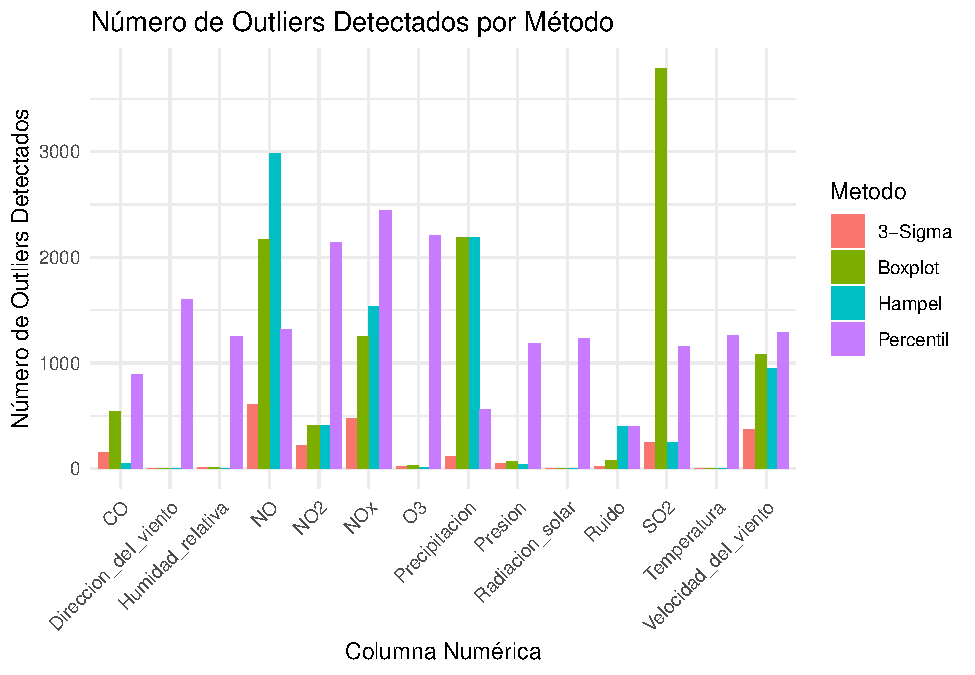
\includegraphics{ProyectoAED2023_plantilla_files/figure-latex/unnamed-chunk-17-1.pdf}

Podemos observar cómo la regla del percentil siempre elimina datos, esto
es debido a la naturaleza de la regla, la cual siempre eliminará el
2.5\% que quede por arriba y el 2.5\% por abajo. Podemos usar esto como
comparador de el resto de métodos.

El resto de métodos, en la mayoría de ocasiones quedan por debajo del
criterio del percentil. No obstante, es visible el agresivo
comportamiento de la regla boxplot y el excesivamente poco agresivo
método de la regla 3-sigma. En cuanto al comportamiento de la regla de
Hampel, parece comportarse como una versión agresiva pero manteniendo la
prudencia de la regla 3-sigma.

Pese a que, según las matemáticas, cuantos más datos tenemos, más se
parece la distribución de los mismos a una Gaussiana, hemos visto
anteriormente que no todos los datos siguen esta distribución.

Por este motivo, hemos decidido utilizar la regla de Hampel para la
detección de los outliers, ya que esta es una regla robusta a
distribuciones que no sean Gaussianas.

A continuación, reemplazaremos los outliers detectados por NA.

\begin{Shaded}
\begin{Highlighting}[]
\NormalTok{datos\_no\_outliers }\OtherTok{\textless{}{-}}\NormalTok{ datos }\SpecialCharTok{\%\textgreater{}\%}
  \FunctionTok{mutate\_at}\NormalTok{(}\FunctionTok{vars}\NormalTok{(}\FunctionTok{all\_of}\NormalTok{(columnas\_numericas)), }\SpecialCharTok{\textasciitilde{}} \FunctionTok{replace\_outliers}\NormalTok{(., hampel))}
\end{Highlighting}
\end{Shaded}

\hypertarget{analisis-bivariante}{%
\section{Analisis bivariante}\label{analisis-bivariante}}

Partiendo de las conclusiones obtenidas en el apartado de análisis de
datos faltantes, nos parece interesante ver si existe alguna influencia
en el valor de la variable por parte de la estación de la que proviene.
En caso de no existir una influencia considerable podemos utilizar los
valores obtenidos en otras estaciones para imputar otros. Finalmente
comprobaremos si año influye en el valor de la variable, para ver si a
lo largo del tiempo ha ocurrido algún cambio considerable.

Mediante boxplots vamos a analizar como se distribuyen los datos
respecto a las estaciones. En primer lugar los gases:

\begin{Shaded}
\begin{Highlighting}[]
\CommentTok{\# Gases}
\NormalTok{datos\_no\_outliers }\SpecialCharTok{\%\textgreater{}\%}
  \FunctionTok{select}\NormalTok{(}\FunctionTok{all\_of}\NormalTok{(variables[}\DecValTok{2}\SpecialCharTok{:}\DecValTok{8}\NormalTok{])) }\SpecialCharTok{\%\textgreater{}\%}
  \FunctionTok{pivot\_longer}\NormalTok{(}\AttributeTok{cols =} \DecValTok{2}\SpecialCharTok{:}\DecValTok{7}\NormalTok{, }\AttributeTok{names\_to =} \StringTok{\textquotesingle{}Variables\textquotesingle{}}\NormalTok{, }\AttributeTok{values\_to =} \StringTok{\textquotesingle{}valor\textquotesingle{}}\NormalTok{, }\AttributeTok{values\_drop\_na =}\NormalTok{ T) }\SpecialCharTok{\%\textgreater{}\%}
  \FunctionTok{ggplot}\NormalTok{(}\FunctionTok{aes}\NormalTok{(}\AttributeTok{y=}\NormalTok{valor, }\AttributeTok{fill=}\NormalTok{Estacion)) }\SpecialCharTok{+} 
  \FunctionTok{geom\_boxplot}\NormalTok{(}\AttributeTok{outlier.size =} \DecValTok{1}\NormalTok{) }\SpecialCharTok{+}
  \FunctionTok{facet\_wrap}\NormalTok{(}\SpecialCharTok{\textasciitilde{}}\NormalTok{Variables, }\AttributeTok{scales =} \StringTok{"free\_y"}\NormalTok{) }\SpecialCharTok{+} 
  \FunctionTok{theme}\NormalTok{(}\AttributeTok{axis.text.x =} \FunctionTok{element\_blank}\NormalTok{(), }\AttributeTok{legend.position =} \StringTok{"none"}\NormalTok{)}
\end{Highlighting}
\end{Shaded}

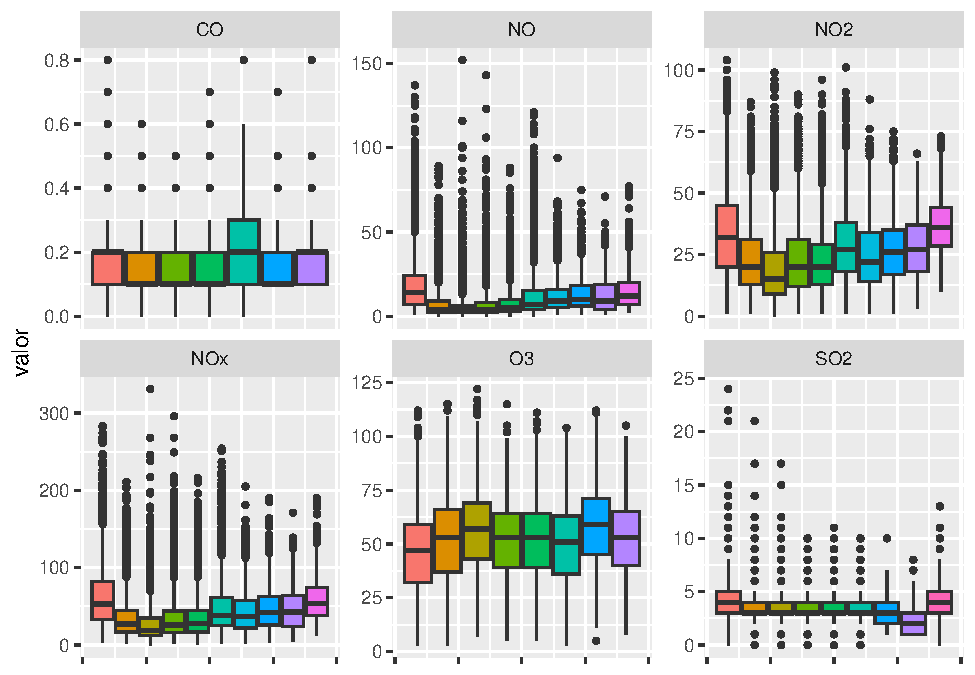
\includegraphics{ProyectoAED2023_plantilla_files/figure-latex/unnamed-chunk-19-1.pdf}

En segundo lugar las variables meteorológicas:

\begin{Shaded}
\begin{Highlighting}[]
\CommentTok{\# Variables meteorológicas y ruido}
\NormalTok{datos\_no\_outliers }\SpecialCharTok{\%\textgreater{}\%}
  \FunctionTok{select}\NormalTok{(}\FunctionTok{all\_of}\NormalTok{(variables[}\FunctionTok{c}\NormalTok{(}\DecValTok{2}\NormalTok{,}\FunctionTok{c}\NormalTok{(}\DecValTok{9}\SpecialCharTok{:}\DecValTok{16}\NormalTok{))])) }\SpecialCharTok{\%\textgreater{}\%}
  \FunctionTok{pivot\_longer}\NormalTok{(}\AttributeTok{cols =} \DecValTok{2}\SpecialCharTok{:}\DecValTok{9}\NormalTok{, }\AttributeTok{names\_to =} \StringTok{\textquotesingle{}Variables\textquotesingle{}}\NormalTok{, }\AttributeTok{values\_to =} \StringTok{\textquotesingle{}valor\textquotesingle{}}\NormalTok{, }\AttributeTok{values\_drop\_na =}\NormalTok{ T) }\SpecialCharTok{\%\textgreater{}\%}
  \FunctionTok{ggplot}\NormalTok{(}\FunctionTok{aes}\NormalTok{(}\AttributeTok{y=}\NormalTok{valor, }\AttributeTok{fill=}\NormalTok{Estacion)) }\SpecialCharTok{+} 
  \FunctionTok{geom\_boxplot}\NormalTok{(}\AttributeTok{outlier.size =} \DecValTok{1}\NormalTok{) }\SpecialCharTok{+}
  \FunctionTok{facet\_wrap}\NormalTok{(}\SpecialCharTok{\textasciitilde{}}\NormalTok{Variables, }\AttributeTok{scales =} \StringTok{"free\_y"}\NormalTok{) }\SpecialCharTok{+} 
  \FunctionTok{theme}\NormalTok{(}\AttributeTok{axis.text.x =} \FunctionTok{element\_blank}\NormalTok{(), }\AttributeTok{legend.position =} \StringTok{"none"}\NormalTok{)}
\end{Highlighting}
\end{Shaded}

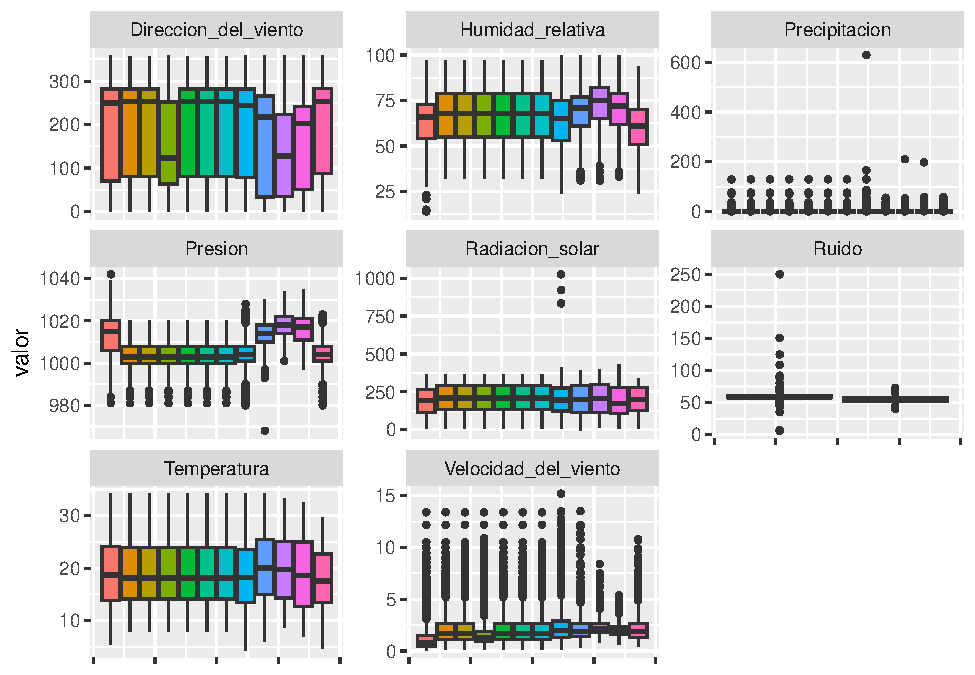
\includegraphics{ProyectoAED2023_plantilla_files/figure-latex/unnamed-chunk-20-1.pdf}

Podemos concluir con que generalmente la estación no influye en los
valores de las variables. Esta información nos es útil para la
imputación de NA's, ya que podemos emplear la media de las medidas
obtenidas por otras estaciones. Respecto al ruido, el cual únicamente se
mide en las estaciones de ``Pista Silla'' y ``Viveros'' si parece tener
un valor un poco mayor en ``Pista Silla''. Esto puede deberse a que esta
estación se encuentra en un lugar con mayor tránsito de coches.

Ahora vamos a ver una sencilla evolución mediante boxplots de el valor
de las variables a lo largo de los años. Comenzamos con los gases:

\begin{Shaded}
\begin{Highlighting}[]
\CommentTok{\# Gases}
\NormalTok{datos\_no\_outliers }\SpecialCharTok{\%\textgreater{}\%}
  \FunctionTok{select}\NormalTok{(}\FunctionTok{all\_of}\NormalTok{(variables[}\FunctionTok{c}\NormalTok{(}\DecValTok{1}\NormalTok{,}\DecValTok{3}\SpecialCharTok{:}\DecValTok{8}\NormalTok{)])) }\SpecialCharTok{\%\textgreater{}\%}
  \FunctionTok{mutate}\NormalTok{(}\AttributeTok{ano =} \FunctionTok{factor}\NormalTok{(}\FunctionTok{year}\NormalTok{(Fecha))) }\SpecialCharTok{\%\textgreater{}\%}
  \FunctionTok{pivot\_longer}\NormalTok{(}\AttributeTok{cols =} \DecValTok{2}\SpecialCharTok{:}\DecValTok{7}\NormalTok{, }\AttributeTok{names\_to =} \StringTok{\textquotesingle{}Variables\textquotesingle{}}\NormalTok{, }\AttributeTok{values\_to =} \StringTok{\textquotesingle{}valor\textquotesingle{}}\NormalTok{, }\AttributeTok{values\_drop\_na =}\NormalTok{ T) }\SpecialCharTok{\%\textgreater{}\%}
  \FunctionTok{ggplot}\NormalTok{(}\FunctionTok{aes}\NormalTok{(}\AttributeTok{y=}\NormalTok{valor, }\AttributeTok{fill=}\NormalTok{ano)) }\SpecialCharTok{+} 
  \FunctionTok{geom\_boxplot}\NormalTok{(}\AttributeTok{outlier.size =} \DecValTok{1}\NormalTok{) }\SpecialCharTok{+}
  \FunctionTok{facet\_wrap}\NormalTok{(}\SpecialCharTok{\textasciitilde{}}\NormalTok{Variables, }\AttributeTok{scales =} \StringTok{"free\_y"}\NormalTok{) }\SpecialCharTok{+} 
  \FunctionTok{theme}\NormalTok{(}\AttributeTok{axis.text.x =} \FunctionTok{element\_blank}\NormalTok{(), }\AttributeTok{legend.position =} \StringTok{"none"}\NormalTok{)}
\end{Highlighting}
\end{Shaded}

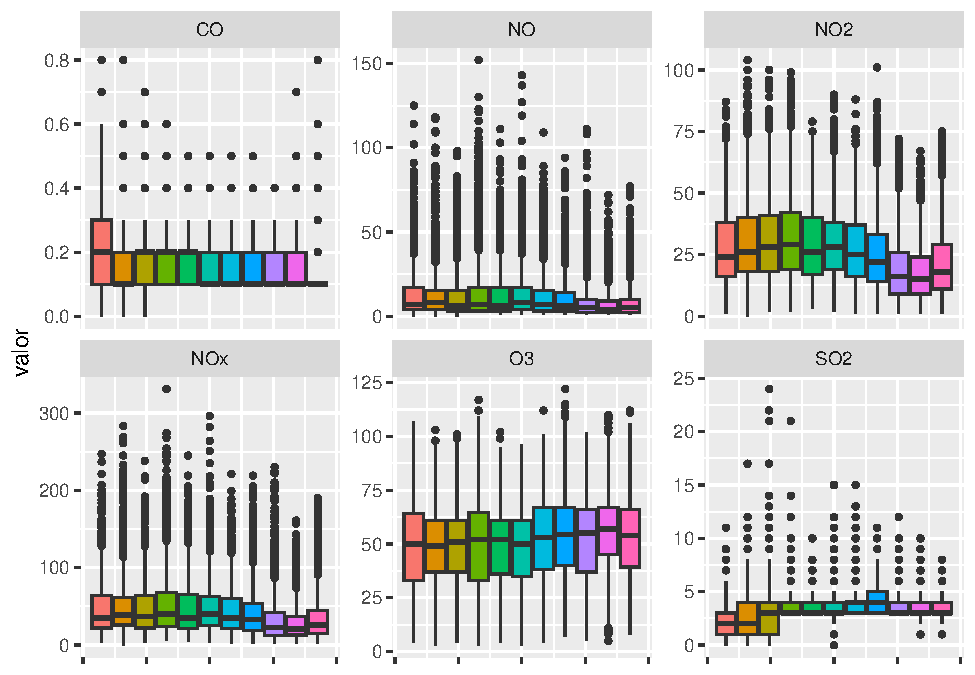
\includegraphics{ProyectoAED2023_plantilla_files/figure-latex/unnamed-chunk-21-1.pdf}

Se puede apreciar una leve reducción a lo largo de los años de los gases
considerados como contaminantes a excepción del SO2 que parece
mantenerse constante. Por otro lado vemos un leve aumento del ozono
(O3), por lo que podría existir una relación con la disminución de gases
contaminantes. Continuamos con las variables meteorológicas:

\begin{Shaded}
\begin{Highlighting}[]
\CommentTok{\# Gases}
\NormalTok{datos\_no\_outliers }\SpecialCharTok{\%\textgreater{}\%}
  \FunctionTok{select}\NormalTok{(}\FunctionTok{all\_of}\NormalTok{(variables[}\FunctionTok{c}\NormalTok{(}\DecValTok{1}\NormalTok{,}\DecValTok{9}\SpecialCharTok{:}\DecValTok{16}\NormalTok{)])) }\SpecialCharTok{\%\textgreater{}\%}
  \FunctionTok{mutate}\NormalTok{(}\AttributeTok{ano =} \FunctionTok{factor}\NormalTok{(}\FunctionTok{year}\NormalTok{(Fecha))) }\SpecialCharTok{\%\textgreater{}\%}
  \FunctionTok{pivot\_longer}\NormalTok{(}\AttributeTok{cols =} \DecValTok{2}\SpecialCharTok{:}\DecValTok{9}\NormalTok{, }\AttributeTok{names\_to =} \StringTok{\textquotesingle{}Variables\textquotesingle{}}\NormalTok{, }\AttributeTok{values\_to =} \StringTok{\textquotesingle{}valor\textquotesingle{}}\NormalTok{, }\AttributeTok{values\_drop\_na =}\NormalTok{ T) }\SpecialCharTok{\%\textgreater{}\%}
  \FunctionTok{ggplot}\NormalTok{(}\FunctionTok{aes}\NormalTok{(}\AttributeTok{y=}\NormalTok{valor, }\AttributeTok{fill=}\NormalTok{ano)) }\SpecialCharTok{+} 
  \FunctionTok{geom\_boxplot}\NormalTok{(}\AttributeTok{outlier.size =} \DecValTok{1}\NormalTok{) }\SpecialCharTok{+}
  \FunctionTok{facet\_wrap}\NormalTok{(}\SpecialCharTok{\textasciitilde{}}\NormalTok{Variables, }\AttributeTok{scales =} \StringTok{"free\_y"}\NormalTok{) }\SpecialCharTok{+} 
  \FunctionTok{theme}\NormalTok{(}\AttributeTok{axis.text.x =} \FunctionTok{element\_blank}\NormalTok{(), }\AttributeTok{legend.position =} \StringTok{"none"}\NormalTok{)}
\end{Highlighting}
\end{Shaded}

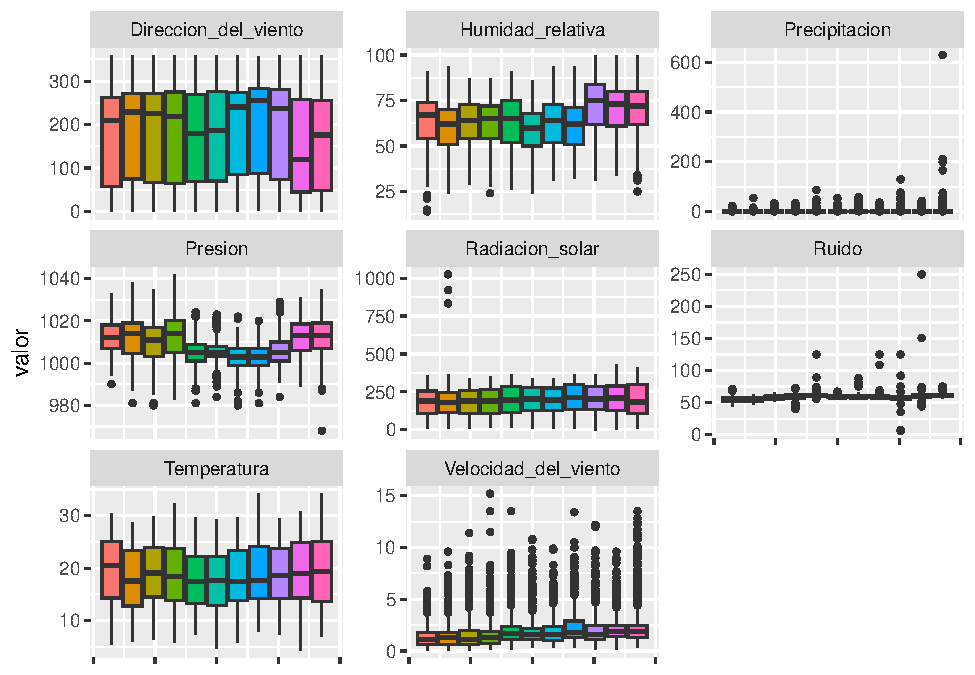
\includegraphics{ProyectoAED2023_plantilla_files/figure-latex/unnamed-chunk-22-1.pdf}

Como era de esperar, las variables meteorológicas no han sufrido
variaciones a lo largo de los años. Por otro lado si que se aprecia un
leve aumento en el ruido.

\hypertarget{imputaciuxf3n-de-nas}{%
\subsection{Imputación de NA's}\label{imputaciuxf3n-de-nas}}

Centrándonos en las variables de interés, si bien son más consistentes
en lo que se refiere a las entradas diarias de cada variable, todavía
hay muchos datos faltantes. No obstante, podemos aprovechar el hecho de
que los datos diarios de las variables en todas las estaciones de
Valencia suelen ser muy parecidos, por lo que decidimos imputar los
datos faltantes en cada día con la media de esta variable sobre todas
las estaciones. Tras realizar esta imputación, todavía hay algunas
variables que presentan NA's, esto se debe a que hay algunos días donde
donde esta variable no se ha medido en ninguna de las estaciones. Esto
sólo ocurre en el 11\% de las observaciones, por lo que decidimos
desprendernos de estas observaciones, ya que el volúmen de datos es
suficientemente grande y los datos todavía pueden considerarse diarios.

\begin{Shaded}
\begin{Highlighting}[]
\NormalTok{imputacion\_NAs }\OtherTok{\textless{}{-}} \ControlFlowTok{function}\NormalTok{(x)\{}
  \FunctionTok{ifelse}\NormalTok{(}\FunctionTok{is.na}\NormalTok{(x), }\FunctionTok{mean}\NormalTok{(x, }\AttributeTok{na.rm =}\NormalTok{ T), x)}
\NormalTok{\}}

\NormalTok{datos\_limpios }\OtherTok{\textless{}{-}}\NormalTok{ datos\_no\_outliers }\SpecialCharTok{\%\textgreater{}\%} 
  \CommentTok{\# Esta hecho arriba}
  \CommentTok{\#filter(Fecha \textgreater{}= as.Date(\textquotesingle{}2012{-}01{-}01\textquotesingle{}, format = \textquotesingle{}\%Y{-}\%m{-}\%d\textquotesingle{}), Fecha \textless{}= as.Date(\textquotesingle{}2022{-}01{-}01\textquotesingle{}, format = \textquotesingle{}\%Y{-}\%m{-}\%d\textquotesingle{})) \%\textgreater{}\%}
  \CommentTok{\#select({-}c(\textquotesingle{}Pb\_(ng/m3)\textquotesingle{},\textquotesingle{}Cd\_(ng/m3)\textquotesingle{},\textquotesingle{}Ni\_(ng/m3)\textquotesingle{},\textquotesingle{}As\_(ng/m3)\textquotesingle{},\textquotesingle{}B(a)p\_(ng/m3)\textquotesingle{},\textquotesingle{}NH3\textquotesingle{},\textquotesingle{}C7H8\textquotesingle{},\textquotesingle{}C6H6\textquotesingle{},\textquotesingle{}C8H10\textquotesingle{})) \%\textgreater{}\% }
  \FunctionTok{group\_by}\NormalTok{(Fecha) }\SpecialCharTok{\%\textgreater{}\%} 
  \FunctionTok{mutate}\NormalTok{(}\FunctionTok{across}\NormalTok{(}\AttributeTok{.cols =} \FunctionTok{all\_of}\NormalTok{(columnas\_numericas), imputacion\_NAs)) }\SpecialCharTok{\%\textgreater{}\%} 
  \FunctionTok{mutate}\NormalTok{(}\FunctionTok{across}\NormalTok{(}\FunctionTok{all\_of}\NormalTok{(columnas\_numericas), reemplazo\_especiales)) }\SpecialCharTok{\%\textgreater{}\%}
\NormalTok{  ungroup}

\DecValTok{100}\SpecialCharTok{*}\FunctionTok{sum}\NormalTok{(}\FunctionTok{complete.cases}\NormalTok{(datos\_limpios))}\SpecialCharTok{/}\FunctionTok{nrow}\NormalTok{(datos\_limpios)}
\end{Highlighting}
\end{Shaded}

\begin{verbatim}
## [1] 87.88126
\end{verbatim}

\begin{Shaded}
\begin{Highlighting}[]
\NormalTok{datos\_limpios }\OtherTok{\textless{}{-}}\NormalTok{ datos\_limpios[}\FunctionTok{complete.cases}\NormalTok{(datos\_limpios),]}
\end{Highlighting}
\end{Shaded}

\hypertarget{correlaciones}{%
\subsection{Correlaciones}\label{correlaciones}}

La correlación puede tener valores en el rango {[}-1,1{]}. Siendo -1 el
indicador de un comportamiento absolutamente contrario y siendo 1 la
misma variable, pues tiene exactamente el mismo comportamiento.

Esto puede darnos información para reflexionar sobre la naturaleza y
comportamiento de los datos.

\begin{Shaded}
\begin{Highlighting}[]
\FunctionTok{library}\NormalTok{(GGally)}

\CommentTok{\# Correlacion Pearson}
\NormalTok{corr1\_P }\OtherTok{\textless{}{-}}\NormalTok{ datos[}\DecValTok{3}\SpecialCharTok{:}\DecValTok{15}\NormalTok{] }\SpecialCharTok{\%\textgreater{}\%}
\NormalTok{  na.omit }\SpecialCharTok{\%\textgreater{}\%}
\NormalTok{  cor}

\NormalTok{corr2\_P }\OtherTok{\textless{}{-}}\NormalTok{ datos\_limpios[}\DecValTok{3}\SpecialCharTok{:}\DecValTok{15}\NormalTok{] }\SpecialCharTok{\%\textgreater{}\%}
\NormalTok{  na.omit }\SpecialCharTok{\%\textgreater{}\%}
\NormalTok{  cor}
\NormalTok{corr2\_P}

\CommentTok{\# Ver diferencias con data raw y data con NA imputados y sin outliers univariantes}
\NormalTok{diff\_P }\OtherTok{\textless{}{-}} \FunctionTok{abs}\NormalTok{(corr1\_P}\SpecialCharTok{{-}}\NormalTok{corr2\_P)}
\NormalTok{diff\_P}

\CommentTok{\# Correlacion Spearman}
\NormalTok{corr1\_S }\OtherTok{\textless{}{-}}\NormalTok{ datos[}\DecValTok{3}\SpecialCharTok{:}\DecValTok{15}\NormalTok{] }\SpecialCharTok{\%\textgreater{}\%}
\NormalTok{  na.omit }\SpecialCharTok{\%\textgreater{}\%}
  \FunctionTok{cor}\NormalTok{(}\AttributeTok{method =} \StringTok{\textquotesingle{}spearman\textquotesingle{}}\NormalTok{)}

\NormalTok{corr2\_S }\OtherTok{\textless{}{-}}\NormalTok{ datos\_limpios[}\DecValTok{3}\SpecialCharTok{:}\DecValTok{15}\NormalTok{] }\SpecialCharTok{\%\textgreater{}\%}
\NormalTok{  na.omit }\SpecialCharTok{\%\textgreater{}\%}
  \FunctionTok{cor}\NormalTok{(}\AttributeTok{method =} \StringTok{\textquotesingle{}spearman\textquotesingle{}}\NormalTok{)}
\NormalTok{corr2\_S}

\NormalTok{diff\_S }\OtherTok{\textless{}{-}} \FunctionTok{abs}\NormalTok{(corr1\_S}\SpecialCharTok{{-}}\NormalTok{corr2\_S)}
\NormalTok{diff\_S}

\FunctionTok{ggcorr}\NormalTok{(datos\_limpios[}\DecValTok{3}\SpecialCharTok{:}\DecValTok{15}\NormalTok{])}
\end{Highlighting}
\end{Shaded}

Basándonos en las observaciones, podemos extraer las siguientes
conclusiones:

\begin{itemize}
\item
  Existe una correlación negativa importante entre NOs y Ozono. Esto
  podría deberse a que la presencia de óxidos de nitrógeno puede
  contribuir a la degradación del ozono en la atmósfera, lo que tiene
  implicaciones para la calidad del aire, la contaminación y el efecto
  hivernadero.
\item
  Correlación positiva de NOx con el resto de NO (NO, NO2\ldots). Como
  era de esperar y como se ha mencionado en la definición de las
  variables, NOx representa el conjunto de oxidos de nitrogeno, entre
  ellos el NO y el NO2.
\item
  Correlación positiva entre Temperatura y Radiación Solar. Esto es
  coherente con las estaciones más cálidas que a menudo experimentan más
  horas de sol y mayor radiación solar.
\item
  Correlación entre Radiación Solar y Ozono. Esto tiene sentido ya que
  la capa de ozono filtra la mayor parte de la radiación ultravioleta
  proveniente del sol, por lo tanto están muy relacionados entre ellos.
\end{itemize}

También hemos filtrado las correlaciones para mostrar únicamente las
mayores correlaciones. Hemos puesto un umbral para escoger solo las
correlaciones que sean mayores a 0.7 para visualizar las variables muy
correlacionadas (eliminando las correlaciones de una variable con ella
misma). Hemos puesto el ejemplo en el que las correlaciones son directas
para la siguiente visualización. Podría realizarse esto para las
correlaciones inversas.

\begin{Shaded}
\begin{Highlighting}[]
\NormalTok{df }\OtherTok{\textless{}{-}} \FunctionTok{cor}\NormalTok{(}\FunctionTok{na.omit}\NormalTok{(datos\_limpios[}\DecValTok{3}\SpecialCharTok{:}\DecValTok{15}\NormalTok{])) }\SpecialCharTok{\%\textgreater{}\%}
  \FunctionTok{as.data.frame}\NormalTok{(.)}

\NormalTok{df}\SpecialCharTok{$}\NormalTok{Variable1 }\OtherTok{\textless{}{-}} \FunctionTok{rownames}\NormalTok{(df)}

\NormalTok{cor }\OtherTok{\textless{}{-}}\NormalTok{ df }\SpecialCharTok{\%\textgreater{}\%}
  \FunctionTok{pivot\_longer}\NormalTok{(}\AttributeTok{cols =} \SpecialCharTok{{-}}\NormalTok{Variable1, }\AttributeTok{names\_to =} \StringTok{"Variable2"}\NormalTok{, }\AttributeTok{values\_to =} \StringTok{"Correlation"}\NormalTok{)}

\NormalTok{correlaciones }\OtherTok{\textless{}{-}}\NormalTok{ cor[cor}\SpecialCharTok{$}\NormalTok{Correlation }\SpecialCharTok{\textgreater{}} \FloatTok{0.7}\NormalTok{,] }\SpecialCharTok{\%\textgreater{}\%} \FunctionTok{arrange}\NormalTok{(}\FunctionTok{desc}\NormalTok{(Correlation)) }\SpecialCharTok{\%\textgreater{}\%} \FunctionTok{filter}\NormalTok{(Variable1 }\SpecialCharTok{!=}\NormalTok{ Variable2)}
\NormalTok{correlaciones\_inversas }\OtherTok{\textless{}{-}}\NormalTok{ cor[cor}\SpecialCharTok{$}\NormalTok{Correlation }\SpecialCharTok{\textless{}} \SpecialCharTok{{-}}\FloatTok{0.7}\NormalTok{,] }\SpecialCharTok{\%\textgreater{}\%} \FunctionTok{arrange}\NormalTok{(Correlation) }\SpecialCharTok{\%\textgreater{}\%} \FunctionTok{filter}\NormalTok{(Variable1 }\SpecialCharTok{!=}\NormalTok{ Variable2)}
\FunctionTok{paste0}\NormalTok{(}\StringTok{"El numero total de correlaciones inversas es "}\NormalTok{,}\FunctionTok{nrow}\NormalTok{(correlaciones\_inversas),}\StringTok{". Por lo tanto, solo estudiaremos las correlaciones directas"}\NormalTok{)}

\FunctionTok{ggplot}\NormalTok{(correlaciones, }\FunctionTok{aes}\NormalTok{(}\AttributeTok{x =}\NormalTok{ Variable1, }\AttributeTok{y =}\NormalTok{ Variable2, }\AttributeTok{color =}\NormalTok{ Correlation)) }\SpecialCharTok{+}
  \FunctionTok{geom\_tile}\NormalTok{(}\FunctionTok{aes}\NormalTok{(}\AttributeTok{fill =}\NormalTok{ Correlation)) }\SpecialCharTok{+}
  \FunctionTok{theme\_minimal}\NormalTok{() }\SpecialCharTok{+}
  \FunctionTok{labs}\NormalTok{(}\AttributeTok{title =} \StringTok{"Correlaciones Positivas"}\NormalTok{)}
\end{Highlighting}
\end{Shaded}

\hypertarget{detecciuxf3n-y-eliminaciuxf3n-de-outliers-con-muxe9todos-multivariable}{%
\subsection{Detección y eliminación de outliers con métodos
multivariable}\label{detecciuxf3n-y-eliminaciuxf3n-de-outliers-con-muxe9todos-multivariable}}

En este apartado, trabajaremos con el dataframe de datos que contiene la
imputación de NA.

\begin{Shaded}
\begin{Highlighting}[]
\NormalTok{distancia\_mahalanobis }\OtherTok{\textless{}{-}} \ControlFlowTok{function}\NormalTok{(x) \{}
\NormalTok{  media }\OtherTok{=} \FunctionTok{colMeans}\NormalTok{(x)}
\NormalTok{  S }\OtherTok{=} \FunctionTok{cov}\NormalTok{(x)}
  
\NormalTok{  dist }\OtherTok{=} \FunctionTok{mahalanobis}\NormalTok{(x,media,S)}
\NormalTok{  umbral }\OtherTok{\textless{}{-}} \FunctionTok{qchisq}\NormalTok{(}\FloatTok{0.95}\NormalTok{, }\AttributeTok{df =} \FunctionTok{ncol}\NormalTok{(x))}

\NormalTok{  outliers }\OtherTok{\textless{}{-}} \FunctionTok{which}\NormalTok{(dist }\SpecialCharTok{\textgreater{}}\NormalTok{ umbral)}
  
  \FunctionTok{return}\NormalTok{(outliers)}
\NormalTok{\}}

\NormalTok{instancias\_outliers }\OtherTok{\textless{}{-}} \FunctionTok{distancia\_mahalanobis}\NormalTok{(datos\_limpios[columnas\_numericas])}
\FunctionTok{paste0}\NormalTok{(}\StringTok{"La distancia de mahalanobis detecta como outliers "}\NormalTok{, }\FunctionTok{length}\NormalTok{(instancias\_outliers),}\StringTok{" datos con una confianza del 95\%. Con estos datos, lo que haremos no es cambiarlos por NA (pues miramos sobre instancias enteras), sino que directamente las eliminaremos."}\NormalTok{)}
\end{Highlighting}
\end{Shaded}

\begin{verbatim}
## [1] "La distancia de mahalanobis detecta como outliers 1937 datos con una confianza del 95%. Con estos datos, lo que haremos no es cambiarlos por NA (pues miramos sobre instancias enteras), sino que directamente las eliminaremos."
\end{verbatim}

\begin{Shaded}
\begin{Highlighting}[]
\NormalTok{datos\_limpios\_sin\_outliers }\OtherTok{\textless{}{-}}\NormalTok{ datos\_limpios[}\SpecialCharTok{{-}}\NormalTok{instancias\_outliers,]}
\end{Highlighting}
\end{Shaded}

\hypertarget{resoluciuxf3n-de-preguntas-planteadas-sobre-los-datos}{%
\section{Resolución de preguntas planteadas sobre los
datos}\label{resoluciuxf3n-de-preguntas-planteadas-sobre-los-datos}}

En esta sección se resolverán las diferentes preguntas planteadas sobre
los datos. \#\# Influencia de carril bici

Para estudiar la influencia de un carril bici por el centro de Valencia,
estudiaremos la evolución de gases contaminantes en diversas estaciones
de la ciudad. Mediremos la evolución de los gases:

\begin{itemize}
\tightlist
\item
  SO2: Originado sobre todo durante la combustión de carburantes
  fósiles.
\item
  NO2: Es un contaminante atmosférico cuyas fuentes fundamentales son el
  tráfico rodado, así como las emisiones de determinadas industrias y
  grandes instalaciones de combustión.
\end{itemize}

Además, las estaciones deberían ser las más céntricas, ya que ahí el
efecto del carril bici y las restricciones de acceso deberían hacerse
más notables. Observaremos las siguientes estaciones:

\begin{itemize}
\tightlist
\item
  Avda. Francia
\item
  Bulevard Sud
\item
  Valencia Centro
\item
  Olivereta
\end{itemize}

\begin{Shaded}
\begin{Highlighting}[]
\NormalTok{datos\_mensuales }\OtherTok{\textless{}{-}}\NormalTok{ datos[}\FunctionTok{c}\NormalTok{(}\StringTok{"Fecha"}\NormalTok{,}\StringTok{"SO2"}\NormalTok{,}\StringTok{"NO2"}\NormalTok{,}\StringTok{"Estacion"}\NormalTok{)] }\SpecialCharTok{\%\textgreater{}\%}
  \FunctionTok{filter}\NormalTok{(Estacion }\SpecialCharTok{\%in\%} \FunctionTok{c}\NormalTok{(}\StringTok{"Avda. Francia"}\NormalTok{,}\StringTok{"Bulevard Sud"}\NormalTok{, }\StringTok{"Valencia Centro"}\NormalTok{, }\StringTok{"Olivereta"}\NormalTok{)) }\SpecialCharTok{\%\textgreater{}\%}
  \FunctionTok{mutate}\NormalTok{(}\AttributeTok{ano =} \FunctionTok{year}\NormalTok{(Fecha), }\AttributeTok{mes =} \FunctionTok{month}\NormalTok{(Fecha)) }\SpecialCharTok{\%\textgreater{}\%}
  \FunctionTok{arrange}\NormalTok{(Fecha) }\SpecialCharTok{\%\textgreater{}\%}
  \FunctionTok{group\_by}\NormalTok{(ano, mes) }\SpecialCharTok{\%\textgreater{}\%}
  \FunctionTok{summarise}\NormalTok{(}\AttributeTok{media\_SO2 =} \FunctionTok{mean}\NormalTok{(SO2, }\AttributeTok{na.rm=}\ConstantTok{TRUE}\NormalTok{), }\AttributeTok{media\_NO2 =} \FunctionTok{mean}\NormalTok{(NO2,}\AttributeTok{na.rm=}\ConstantTok{TRUE}\NormalTok{), }\AttributeTok{.groups=}\StringTok{"drop"}\NormalTok{)}

\FunctionTok{ggplot}\NormalTok{(}\AttributeTok{data =}\NormalTok{ datos\_mensuales, }\FunctionTok{aes}\NormalTok{(}\AttributeTok{x =}\NormalTok{ mes, }\AttributeTok{y =}\NormalTok{ media\_SO2, }\AttributeTok{group =}\NormalTok{ ano, }\AttributeTok{color =} \FunctionTok{factor}\NormalTok{(ano))) }\SpecialCharTok{+}
  \FunctionTok{geom\_line}\NormalTok{() }\SpecialCharTok{+}
  \FunctionTok{labs}\NormalTok{(}\AttributeTok{x =} \StringTok{"Mes"}\NormalTok{, }\AttributeTok{y =} \StringTok{"Media SO2"}\NormalTok{, }\AttributeTok{title =} \StringTok{"Media Mensual SO2 por Año"}\NormalTok{) }\SpecialCharTok{+}
  \FunctionTok{scale\_color\_discrete}\NormalTok{(}\AttributeTok{name =} \StringTok{"Año"}\NormalTok{) }\SpecialCharTok{+}
  \FunctionTok{scale\_x\_continuous}\NormalTok{(}\AttributeTok{breaks =} \DecValTok{1}\SpecialCharTok{:}\DecValTok{12}\NormalTok{, }\AttributeTok{labels =}\NormalTok{ month.abb, }\AttributeTok{limits =} \FunctionTok{c}\NormalTok{(}\DecValTok{1}\NormalTok{, }\DecValTok{12}\NormalTok{)) }\SpecialCharTok{+}
  \FunctionTok{theme\_minimal}\NormalTok{() }\SpecialCharTok{+}
  \FunctionTok{theme}\NormalTok{(}\AttributeTok{axis.text.x =} \FunctionTok{element\_text}\NormalTok{(}\AttributeTok{angle =} \DecValTok{45}\NormalTok{, }\AttributeTok{hjust =} \DecValTok{1}\NormalTok{))}
\end{Highlighting}
\end{Shaded}

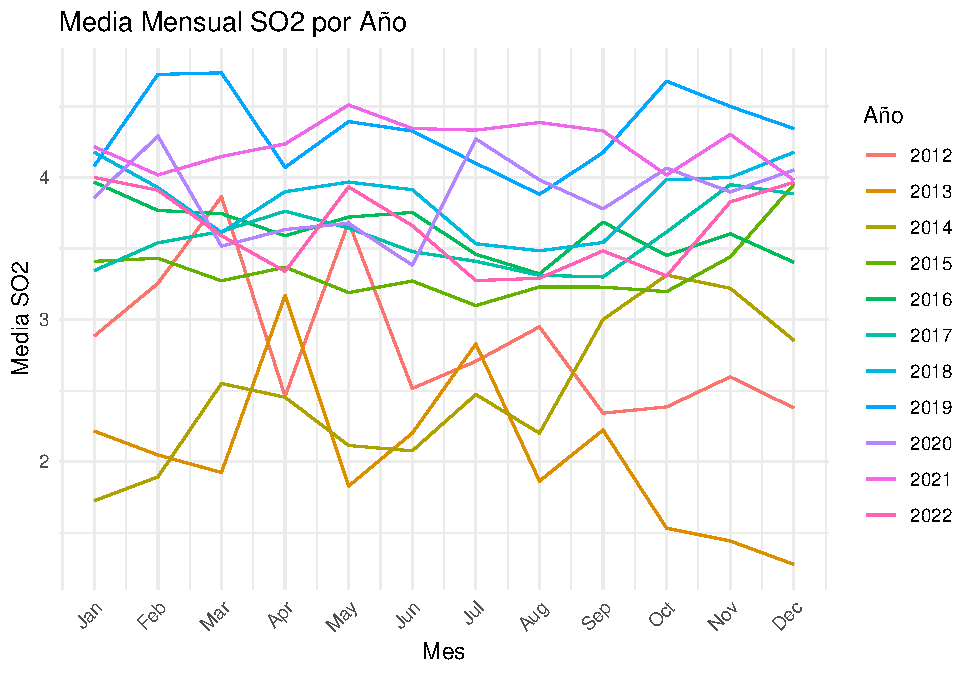
\includegraphics{ProyectoAED2023_plantilla_files/figure-latex/unnamed-chunk-27-1.pdf}

\begin{Shaded}
\begin{Highlighting}[]
\FunctionTok{ggplot}\NormalTok{(}\AttributeTok{data =}\NormalTok{ datos\_mensuales, }\FunctionTok{aes}\NormalTok{(}\AttributeTok{x =}\NormalTok{ mes, }\AttributeTok{y =}\NormalTok{ media\_NO2, }\AttributeTok{group =}\NormalTok{ ano, }\AttributeTok{color =} \FunctionTok{factor}\NormalTok{(ano))) }\SpecialCharTok{+}
  \FunctionTok{geom\_line}\NormalTok{() }\SpecialCharTok{+}
  \FunctionTok{labs}\NormalTok{(}\AttributeTok{x =} \StringTok{"Mes"}\NormalTok{, }\AttributeTok{y =} \StringTok{"Media NO2"}\NormalTok{, }\AttributeTok{title =} \StringTok{"Media Mensual NO2 por Año"}\NormalTok{) }\SpecialCharTok{+}
  \FunctionTok{scale\_color\_discrete}\NormalTok{(}\AttributeTok{name =} \StringTok{"Año"}\NormalTok{) }\SpecialCharTok{+}
  \FunctionTok{scale\_x\_continuous}\NormalTok{(}\AttributeTok{breaks =} \DecValTok{1}\SpecialCharTok{:}\DecValTok{12}\NormalTok{, }\AttributeTok{labels =}\NormalTok{ month.abb, }\AttributeTok{limits =} \FunctionTok{c}\NormalTok{(}\DecValTok{1}\NormalTok{, }\DecValTok{12}\NormalTok{)) }\SpecialCharTok{+}
  \FunctionTok{theme\_minimal}\NormalTok{() }\SpecialCharTok{+}
  \FunctionTok{theme}\NormalTok{(}\AttributeTok{axis.text.x =} \FunctionTok{element\_text}\NormalTok{(}\AttributeTok{angle =} \DecValTok{45}\NormalTok{, }\AttributeTok{hjust =} \DecValTok{1}\NormalTok{))}
\end{Highlighting}
\end{Shaded}

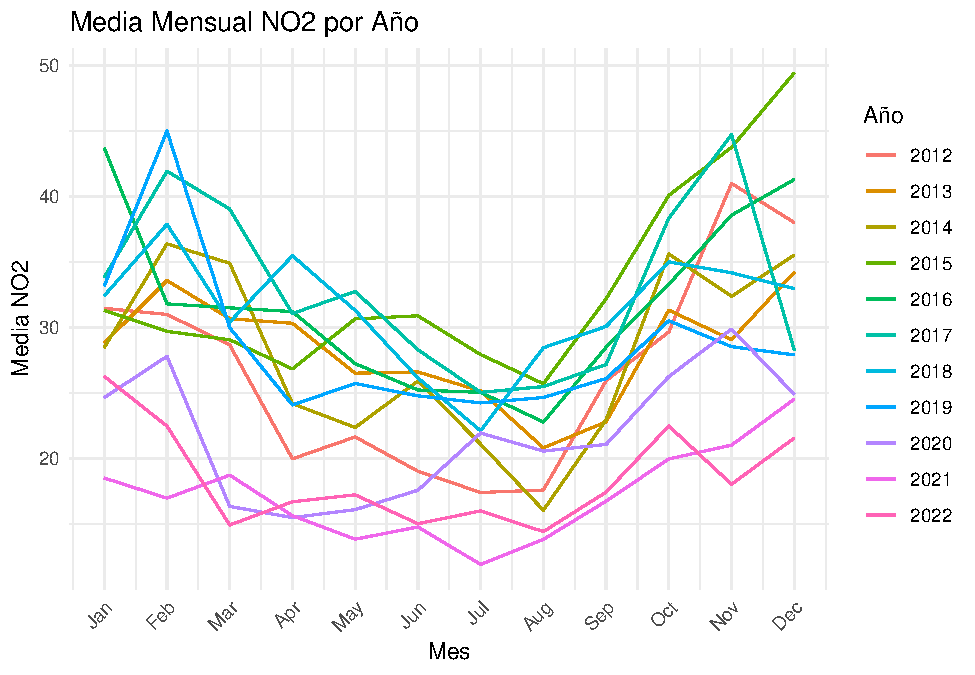
\includegraphics{ProyectoAED2023_plantilla_files/figure-latex/unnamed-chunk-27-2.pdf}

NOTA: El gráfico de NO2 se ve mucho mejor la reducción cuando se
observan todas las estaciones.

Si bien no se observan cambios significativos en los niveles de SO2, en
los niveles de NO2 sí que podemos observar una evolución.

Respecto al NO2 si que se puede apreciar una reducción a lo largo de los
años. Con unos niveles más bajos especialmente en los últimos 3 años.
Además se puede apreciar una periodicidad, concretamente una reducción
de los niveles de NO2 en los meses de verano. Esto coincide con el
momento del año donde menos gente vive en la ciudad y por lo tanto menos
tráfico hay. En conclusión parece que las medidas de transporte que se
han tomado en la ciudad han influenciado en la reducción de gases
contaminantes.

\hypertarget{relaciuxf3n-entre-la-calidad-del-aire-y-el-dia-de-la-semana}{%
\subsection{Relación entre la calidad del aire y el dia de la
semana}\label{relaciuxf3n-entre-la-calidad-del-aire-y-el-dia-de-la-semana}}

Aqui observamos si, en general la calidad del aire se ve influenciada
por el día de la semana. Queremos sobre todo fijarnos en la distinción
entre días laborables y de descanso. Podemos comprobar cómo,
efectivamente, existe una disminución en los gases contaminantes los
días festivos con respecto a los días laborables.

\begin{Shaded}
\begin{Highlighting}[]
\NormalTok{gases\_interes }\OtherTok{\textless{}{-}} \FunctionTok{c}\NormalTok{(}\StringTok{"NO"}\NormalTok{,}\StringTok{"NO2"}\NormalTok{,}\StringTok{"NOx"}\NormalTok{,}\StringTok{"SO2"}\NormalTok{,}\StringTok{"CO"}\NormalTok{)}

\NormalTok{datos\_semanales }\OtherTok{\textless{}{-}}\NormalTok{ datos\_limpios }\SpecialCharTok{\%\textgreater{}\%}
  \FunctionTok{mutate}\NormalTok{(}\AttributeTok{Dia\_de\_la\_semana =} \FunctionTok{factor}\NormalTok{(}\FunctionTok{wday}\NormalTok{(Fecha))) }\SpecialCharTok{\%\textgreater{}\%}
  \FunctionTok{filter}\NormalTok{(}\SpecialCharTok{!}\NormalTok{(Dia\_de\_la\_semana }\SpecialCharTok{\%in\%} \FunctionTok{c}\NormalTok{(}\DecValTok{1}\NormalTok{,}\DecValTok{6}\NormalTok{))) }\SpecialCharTok{\%\textgreater{}\%}
  \FunctionTok{select}\NormalTok{(gases\_interes) }\SpecialCharTok{\%\textgreater{}\%}
  \FunctionTok{summarise\_all}\NormalTok{(}\AttributeTok{.funs =} \FunctionTok{list}\NormalTok{(mean)) }\SpecialCharTok{\%\textgreater{}\%}
  \FunctionTok{pivot\_longer}\NormalTok{(}\AttributeTok{cols=}\FunctionTok{everything}\NormalTok{(),}\AttributeTok{names\_to =} \StringTok{"Gas"}\NormalTok{,}\AttributeTok{values\_to=}\StringTok{"Valor"}\NormalTok{)}

\NormalTok{datos\_festivos }\OtherTok{\textless{}{-}}\NormalTok{ datos\_limpios }\SpecialCharTok{\%\textgreater{}\%}
  \FunctionTok{mutate}\NormalTok{(}\AttributeTok{Dia\_de\_la\_semana =} \FunctionTok{factor}\NormalTok{(}\FunctionTok{wday}\NormalTok{(Fecha))) }\SpecialCharTok{\%\textgreater{}\%}
  \FunctionTok{filter}\NormalTok{(Dia\_de\_la\_semana }\SpecialCharTok{\%in\%} \FunctionTok{c}\NormalTok{(}\DecValTok{1}\NormalTok{,}\DecValTok{6}\NormalTok{)) }\SpecialCharTok{\%\textgreater{}\%}
  \FunctionTok{select}\NormalTok{(gases\_interes) }\SpecialCharTok{\%\textgreater{}\%}
  \FunctionTok{summarise\_all}\NormalTok{(}\AttributeTok{.funs =} \FunctionTok{list}\NormalTok{(mean)) }\SpecialCharTok{\%\textgreater{}\%}
  \FunctionTok{pivot\_longer}\NormalTok{(}\AttributeTok{cols=}\FunctionTok{everything}\NormalTok{(),}\AttributeTok{names\_to =} \StringTok{"Gas"}\NormalTok{,}\AttributeTok{values\_to=}\StringTok{"Valor"}\NormalTok{)}

\NormalTok{datos\_combinados }\OtherTok{\textless{}{-}} \FunctionTok{rbind}\NormalTok{(}
  \FunctionTok{transform}\NormalTok{(datos\_semanales, }\AttributeTok{Tipo =} \StringTok{"Semanal"}\NormalTok{),}
  \FunctionTok{transform}\NormalTok{(datos\_festivos, }\AttributeTok{Tipo =} \StringTok{"Festivo"}\NormalTok{)}
\NormalTok{)}

\FunctionTok{ggplot}\NormalTok{(datos\_combinados, }\FunctionTok{aes}\NormalTok{(}\AttributeTok{x =}\NormalTok{ Gas, }\AttributeTok{y =}\NormalTok{ Valor, }\AttributeTok{fill =}\NormalTok{ Tipo)) }\SpecialCharTok{+}
  \FunctionTok{geom\_bar}\NormalTok{(}\AttributeTok{stat =} \StringTok{"identity"}\NormalTok{, }\AttributeTok{position =} \FunctionTok{position\_dodge}\NormalTok{()) }\SpecialCharTok{+}
  \FunctionTok{labs}\NormalTok{(}\AttributeTok{title =} \StringTok{"Valores de Gases Semanales y Festivos"}\NormalTok{,}
       \AttributeTok{x =} \StringTok{"Gas"}\NormalTok{,}
       \AttributeTok{y =} \StringTok{"Valor"}\NormalTok{) }\SpecialCharTok{+}
  \FunctionTok{scale\_fill\_manual}\NormalTok{(}\AttributeTok{values =} \FunctionTok{c}\NormalTok{(}\StringTok{"Semanal"} \OtherTok{=} \StringTok{"blue"}\NormalTok{, }\StringTok{"Festivo"} \OtherTok{=} \StringTok{"red"}\NormalTok{)) }\SpecialCharTok{+}
  \FunctionTok{theme\_minimal}\NormalTok{() }\SpecialCharTok{+}
  \FunctionTok{theme}\NormalTok{(}\AttributeTok{legend.title =} \FunctionTok{element\_blank}\NormalTok{())}
\end{Highlighting}
\end{Shaded}

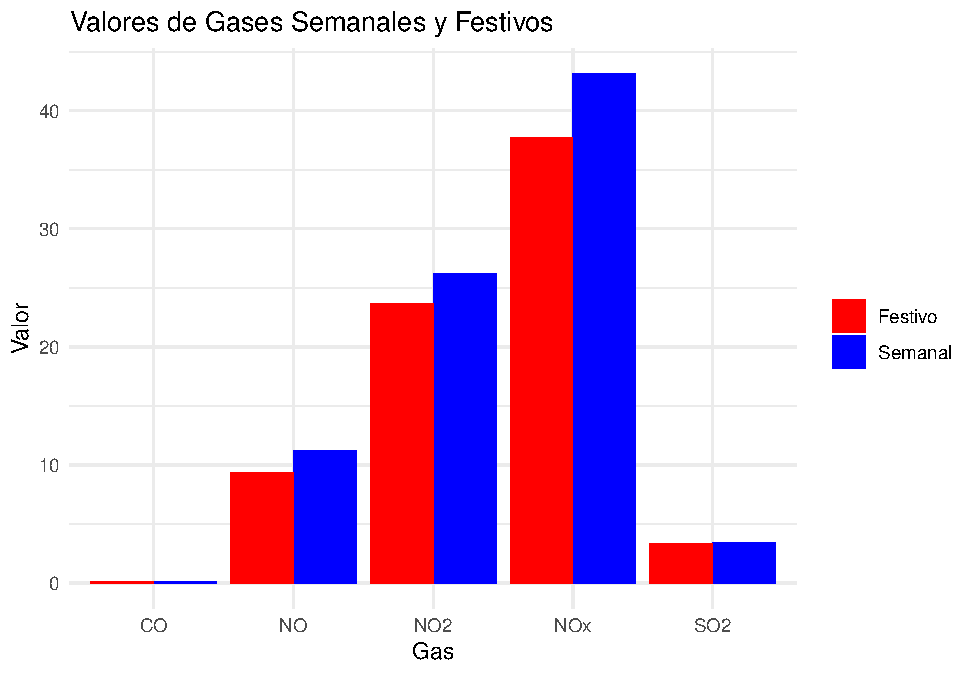
\includegraphics{ProyectoAED2023_plantilla_files/figure-latex/unnamed-chunk-28-1.pdf}

\hypertarget{evoluciuxf3n-de-la-contaminaciuxf3n-sonora-a-lo-largo-de-los-auxf1os}{%
\subsection{Evolución de la contaminación sonora a lo largo de los
años}\label{evoluciuxf3n-de-la-contaminaciuxf3n-sonora-a-lo-largo-de-los-auxf1os}}

Podemos observar un incremento visibleen la medición del ruido medio a
lo largo de los años. Obviamente, en los datos del 2020 podemos observar
un decrecimiento de los mismos, producto del parón de la pandemia, pero
vemos cómo continúa aun así subiendo.

\begin{Shaded}
\begin{Highlighting}[]
\NormalTok{datos\_ruido }\OtherTok{\textless{}{-}}\NormalTok{ datos\_limpios[}\FunctionTok{c}\NormalTok{(}\StringTok{"Fecha"}\NormalTok{,}\StringTok{"Ruido"}\NormalTok{)] }\SpecialCharTok{\%\textgreater{}\%}
  \FunctionTok{mutate}\NormalTok{(}\AttributeTok{Ano =} \FunctionTok{year}\NormalTok{(Fecha)) }\SpecialCharTok{\%\textgreater{}\%}
  \FunctionTok{select}\NormalTok{(}\SpecialCharTok{{-}}\NormalTok{Fecha) }\SpecialCharTok{\%\textgreater{}\%}
  \FunctionTok{group\_by}\NormalTok{(Ano) }\SpecialCharTok{\%\textgreater{}\%}
  \FunctionTok{summarize}\NormalTok{(}\AttributeTok{Media\_Ruido =} \FunctionTok{mean}\NormalTok{(Ruido, }\AttributeTok{na.rm =} \ConstantTok{TRUE}\NormalTok{, }\AttributeTok{.groups =} \StringTok{"drop"}\NormalTok{))}

\FunctionTok{ggplot}\NormalTok{(datos\_ruido, }\FunctionTok{aes}\NormalTok{(}\AttributeTok{x =}\NormalTok{ Ano, }\AttributeTok{y =}\NormalTok{ Media\_Ruido)) }\SpecialCharTok{+}
  \FunctionTok{geom\_line}\NormalTok{() }\SpecialCharTok{+}
  \FunctionTok{labs}\NormalTok{(}\AttributeTok{x =} \StringTok{"Año"}\NormalTok{, }\AttributeTok{y =} \StringTok{"Media de Ruido"}\NormalTok{) }\SpecialCharTok{+}
  \FunctionTok{theme\_minimal}\NormalTok{() }\SpecialCharTok{+}
  \FunctionTok{scale\_y\_continuous}\NormalTok{(}\AttributeTok{limits =} \FunctionTok{c}\NormalTok{(}\FunctionTok{min}\NormalTok{(datos\_ruido}\SpecialCharTok{$}\NormalTok{Media\_Ruido), }\FunctionTok{max}\NormalTok{(datos\_ruido}\SpecialCharTok{$}\NormalTok{Media\_Ruido)))}
\end{Highlighting}
\end{Shaded}

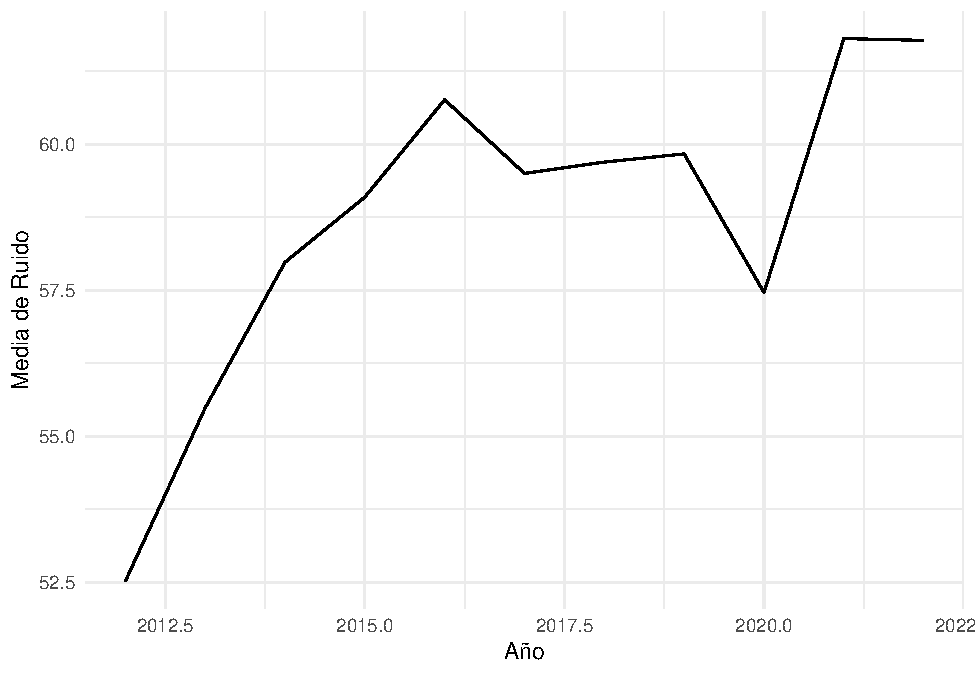
\includegraphics{ProyectoAED2023_plantilla_files/figure-latex/unnamed-chunk-29-1.pdf}

Ahora comprobaremos si este ruido medido depende de la zona dónde la
midamos. Para ello, vamos a observar el comportamiento de la varianza de
la media de los ruidos agrupados por estaciones. Calcularemos la
desviación para cada año y, finalmente, la media de todas las
desviaciones Si el valor es pequeño, entonces podemos afirmar que el
incremento en el ruido no es de ciertas zonas, sino generalizado.

\begin{Shaded}
\begin{Highlighting}[]
\NormalTok{datos\_ruido\_estaciones }\OtherTok{\textless{}{-}}\NormalTok{ datos\_limpios[}\FunctionTok{c}\NormalTok{(}\StringTok{"Fecha"}\NormalTok{,}\StringTok{"Estacion"}\NormalTok{,}\StringTok{"Ruido"}\NormalTok{)] }\SpecialCharTok{\%\textgreater{}\%}
  \FunctionTok{mutate}\NormalTok{(}\AttributeTok{Ano =} \FunctionTok{year}\NormalTok{(Fecha)) }\SpecialCharTok{\%\textgreater{}\%}
  \FunctionTok{select}\NormalTok{(}\SpecialCharTok{{-}}\NormalTok{Fecha) }\SpecialCharTok{\%\textgreater{}\%}
  \FunctionTok{group\_by}\NormalTok{(Ano,Estacion) }\SpecialCharTok{\%\textgreater{}\%}
  \FunctionTok{summarize}\NormalTok{(}\AttributeTok{Media\_Ruido =} \FunctionTok{mean}\NormalTok{(Ruido, }\AttributeTok{na.rm =} \ConstantTok{TRUE}\NormalTok{, }\AttributeTok{.groups =} \StringTok{"drop"}\NormalTok{)) }\SpecialCharTok{\%\textgreater{}\%}
  \FunctionTok{group\_by}\NormalTok{(Ano) }\SpecialCharTok{\%\textgreater{}\%}
  \FunctionTok{summarize}\NormalTok{(}\AttributeTok{Desviacion\_por\_ano =} \FunctionTok{sd}\NormalTok{(Media\_Ruido,}\AttributeTok{na.rm=}\ConstantTok{TRUE}\NormalTok{))}
\end{Highlighting}
\end{Shaded}

\begin{verbatim}
## `summarise()` has grouped output by 'Ano'. You can override using the `.groups`
## argument.
\end{verbatim}

\begin{Shaded}
\begin{Highlighting}[]
\FunctionTok{ggplot}\NormalTok{(datos\_ruido\_estaciones, }\FunctionTok{aes}\NormalTok{(}\AttributeTok{x =}\NormalTok{ Ano, }\AttributeTok{y =}\NormalTok{ Desviacion\_por\_ano)) }\SpecialCharTok{+}
  \FunctionTok{geom\_line}\NormalTok{() }\SpecialCharTok{+}
  \FunctionTok{labs}\NormalTok{(}\AttributeTok{x =} \StringTok{"Año"}\NormalTok{, }\AttributeTok{y =} \StringTok{"Desviacion de ruido por estación"}\NormalTok{) }\SpecialCharTok{+}
  \FunctionTok{theme\_minimal}\NormalTok{() }
\end{Highlighting}
\end{Shaded}

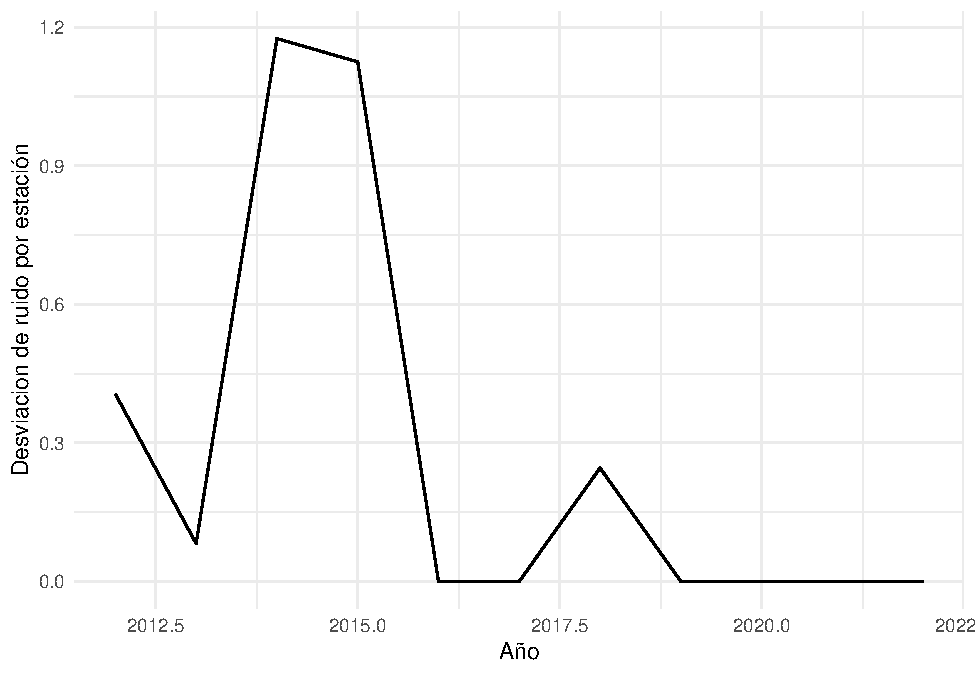
\includegraphics{ProyectoAED2023_plantilla_files/figure-latex/unnamed-chunk-30-1.pdf}

\begin{Shaded}
\begin{Highlighting}[]
\FunctionTok{mean}\NormalTok{(datos\_ruido\_estaciones}\SpecialCharTok{$}\NormalTok{Desviacion\_por\_ano)}
\end{Highlighting}
\end{Shaded}

\begin{verbatim}
## [1] 0.2758076
\end{verbatim}

Podemos observar que, para los valores que tratamos (sobre 50 y 60), una
desviación del 0.3 es despreciable.

\hypertarget{evoluciuxf3n-de-la-temperatura-a-lo-largo-de-los-auxf1os}{%
\subsection{Evolución de la temperatura a lo largo de los
años}\label{evoluciuxf3n-de-la-temperatura-a-lo-largo-de-los-auxf1os}}

También se puede observar el aumento generalizado de la temperatura a lo
largo de los años. Es curioso que, pese a que en el mundo existe un
aumento generalizado de la temperatura, en Valencia estuvo bajando esta
tendencia y no es hasta el año 2017 que comenzaron a subir de nuevo.
Pese a lo mencionado, bastante visible el hecho de que nos encontramos
en una tendencia creciente.

\begin{Shaded}
\begin{Highlighting}[]
\NormalTok{datos\_temperatura }\OtherTok{\textless{}{-}}\NormalTok{ datos\_limpios[}\FunctionTok{c}\NormalTok{(}\StringTok{"Fecha"}\NormalTok{,}\StringTok{"Temperatura"}\NormalTok{)] }\SpecialCharTok{\%\textgreater{}\%}
  \FunctionTok{mutate}\NormalTok{(}\AttributeTok{Ano =} \FunctionTok{year}\NormalTok{(Fecha)) }\SpecialCharTok{\%\textgreater{}\%}
  \FunctionTok{select}\NormalTok{(}\SpecialCharTok{{-}}\NormalTok{Fecha) }\SpecialCharTok{\%\textgreater{}\%}
  \FunctionTok{group\_by}\NormalTok{(Ano) }\SpecialCharTok{\%\textgreater{}\%}
  \FunctionTok{summarize}\NormalTok{(}\AttributeTok{Media\_Temperatura =} \FunctionTok{mean}\NormalTok{(Temperatura, }\AttributeTok{na.rm =} \ConstantTok{TRUE}\NormalTok{, }\AttributeTok{.groups =} \StringTok{"drop"}\NormalTok{))}

\FunctionTok{ggplot}\NormalTok{(datos\_temperatura, }\FunctionTok{aes}\NormalTok{(}\AttributeTok{x =}\NormalTok{ Ano, }\AttributeTok{y =}\NormalTok{ Media\_Temperatura)) }\SpecialCharTok{+}
  \FunctionTok{geom\_line}\NormalTok{() }\SpecialCharTok{+}
  \FunctionTok{labs}\NormalTok{(}\AttributeTok{x =} \StringTok{"Año"}\NormalTok{, }\AttributeTok{y =} \StringTok{"Media de Temperatura"}\NormalTok{) }\SpecialCharTok{+}
  \FunctionTok{theme\_minimal}\NormalTok{() }\SpecialCharTok{+}
  \FunctionTok{scale\_y\_continuous}\NormalTok{(}\AttributeTok{limits =} \FunctionTok{c}\NormalTok{(}\FunctionTok{min}\NormalTok{(datos\_temperatura}\SpecialCharTok{$}\NormalTok{Media\_Temperatura), }\FunctionTok{max}\NormalTok{(datos\_temperatura}\SpecialCharTok{$}\NormalTok{Media\_Temperatura)))}
\end{Highlighting}
\end{Shaded}

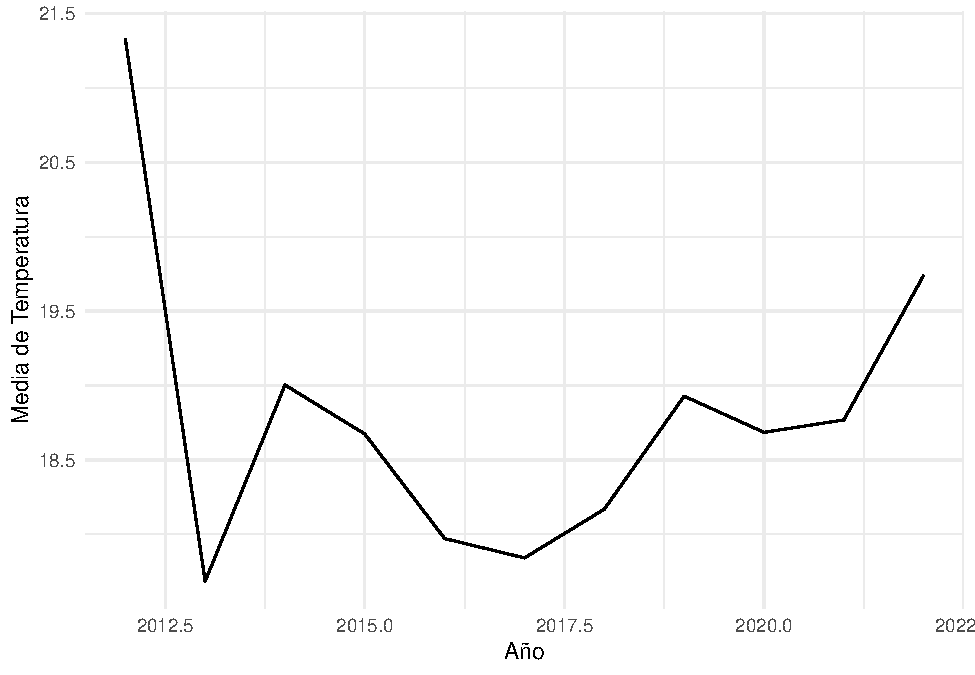
\includegraphics{ProyectoAED2023_plantilla_files/figure-latex/unnamed-chunk-31-1.pdf}

\hypertarget{cuxf3mo-se-ha-comportado-la-contaminaciuxf3n-a-lo-largo-de-los-auxf1os}{%
\subsection{Cómo se ha comportado la contaminación a lo largo de los
años}\label{cuxf3mo-se-ha-comportado-la-contaminaciuxf3n-a-lo-largo-de-los-auxf1os}}

Cuando contestamos a la primera pregunta, nos centramos en gases que
soltaban los carburantes y solo observamos las estaciones más cercanas
al centro de Valencia. En esta ocasión, estudiaremos el comportamiento
de todos los gases contaminantes en todas las estaciones.

Esta vez podemos observar que se produjo un pico de todos los gases en
el año 2016, pero que por lo general las medidas de estos se han
mantenido bastante estables o incluso decrecientes en el tiempo.

\begin{Shaded}
\begin{Highlighting}[]
\NormalTok{datos\_gases }\OtherTok{\textless{}{-}}\NormalTok{ datos\_limpios[}\FunctionTok{c}\NormalTok{(}\StringTok{"Fecha"}\NormalTok{, }\StringTok{"NO"}\NormalTok{, }\StringTok{"NO2"}\NormalTok{, }\StringTok{"NOx"}\NormalTok{, }\StringTok{"SO2"}\NormalTok{, }\StringTok{"CO"}\NormalTok{)] }\SpecialCharTok{\%\textgreater{}\%}
  \FunctionTok{mutate}\NormalTok{(}\AttributeTok{Ano =} \FunctionTok{year}\NormalTok{(Fecha)) }\SpecialCharTok{\%\textgreater{}\%}
  \FunctionTok{select}\NormalTok{(}\SpecialCharTok{{-}}\NormalTok{Fecha) }\SpecialCharTok{\%\textgreater{}\%}
  \FunctionTok{pivot\_longer}\NormalTok{(}\AttributeTok{cols =} \FunctionTok{c}\NormalTok{(}\StringTok{"NO"}\NormalTok{, }\StringTok{"NO2"}\NormalTok{, }\StringTok{"NOx"}\NormalTok{, }\StringTok{"SO2"}\NormalTok{, }\StringTok{"CO"}\NormalTok{), }\AttributeTok{names\_to =} \StringTok{"Gas"}\NormalTok{, }\AttributeTok{values\_to =} \StringTok{"Valor"}\NormalTok{) }\SpecialCharTok{\%\textgreater{}\%}
  \FunctionTok{group\_by}\NormalTok{(Ano, Gas) }\SpecialCharTok{\%\textgreater{}\%}
  \FunctionTok{summarize}\NormalTok{(}\AttributeTok{Media =} \FunctionTok{mean}\NormalTok{(Valor, }\AttributeTok{na.rm =} \ConstantTok{TRUE}\NormalTok{, }\AttributeTok{.groups =} \StringTok{"drop"}\NormalTok{))}
\end{Highlighting}
\end{Shaded}

\begin{verbatim}
## `summarise()` has grouped output by 'Ano'. You can override using the `.groups`
## argument.
\end{verbatim}

\begin{Shaded}
\begin{Highlighting}[]
\FunctionTok{ggplot}\NormalTok{(datos\_gases, }\FunctionTok{aes}\NormalTok{(}\AttributeTok{x=}\NormalTok{Ano,}\AttributeTok{y=}\NormalTok{Media,}\AttributeTok{color=}\NormalTok{Gas)) }\SpecialCharTok{+} 
  \FunctionTok{geom\_line}\NormalTok{() }\SpecialCharTok{+}
  \FunctionTok{labs}\NormalTok{(}\AttributeTok{x =} \StringTok{"Año"}\NormalTok{) }\SpecialCharTok{+}
  \FunctionTok{theme\_minimal}\NormalTok{()}
\end{Highlighting}
\end{Shaded}

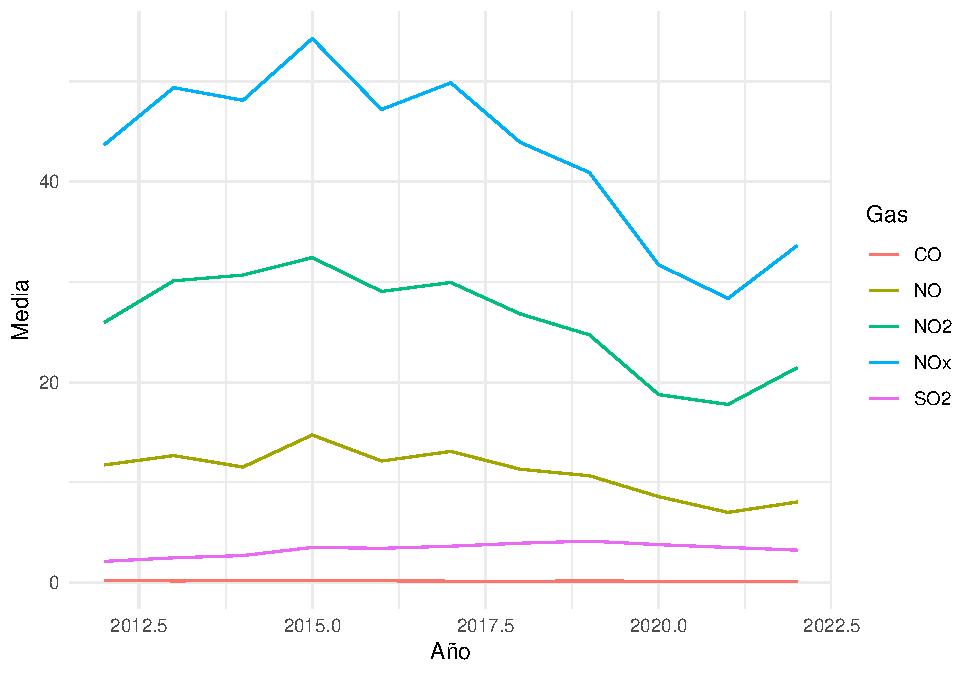
\includegraphics{ProyectoAED2023_plantilla_files/figure-latex/unnamed-chunk-32-1.pdf}

%%%%%%%%%%%%%%%%%%%%%%%%%%%%%%%%%%%%%%%%%%

\vspace{6pt}

%%%%%%%%%%%%%%%%%%%%%%%%%%%%%%%%%%%%%%%%%%
%% optional

% Only for the journal Methods and Protocols:
% If you wish to submit a video article, please do so with any other supplementary material.
% \supplementary{The following supporting information can be downloaded at: \linksupplementary{s1}, Figure S1: title; Table S1: title; Video S1: title. A supporting video article is available at doi: link.}

%%%%%%%%%%%%%%%%%%%%%%%%%%%%%%%%%%%%%%%%%%







%%%%%%%%%%%%%%%%%%%%%%%%%%%%%%%%%%%%%%%%%%
%% Optional

%% Only for journal Encyclopedia

\abbreviations{Abbreviations}{
The following abbreviations are used in this manuscript:\\

\noindent
\begin{tabular}{@{}ll}
MDPI & Multidisciplinary Digital Publishing Institute \\
DOAJ & Directory of open access journals \\
TLA & Three letter acronym \\
LD & linear dichroism \\
\end{tabular}}

%%%%%%%%%%%%%%%%%%%%%%%%%%%%%%%%%%%%%%%%%%
%% Optional
%%%%%%%%%%%%%%%%%%%%%%%%%%%%%%%%%%%%%%%%%%
\begin{adjustwidth}{-\extralength}{0cm}

%\printendnotes[custom] % Un-comment to print a list of endnotes



% If authors have biography, please use the format below
%\section*{Short Biography of Authors}
%\bio
%{\raisebox{-0.35cm}{\includegraphics[width=3.5cm,height=5.3cm,clip,keepaspectratio]{Definitions/author1.pdf}}}
%{\textbf{Firstname Lastname} Biography of first author}
%
%\bio
%{\raisebox{-0.35cm}{\includegraphics[width=3.5cm,height=5.3cm,clip,keepaspectratio]{Definitions/author2.jpg}}}
%{\textbf{Firstname Lastname} Biography of second author}

%%%%%%%%%%%%%%%%%%%%%%%%%%%%%%%%%%%%%%%%%%
%% for journal Sci
%\reviewreports{\\
%Reviewer 1 comments and authors’ response\\
%Reviewer 2 comments and authors’ response\\
%Reviewer 3 comments and authors’ response
%}
%%%%%%%%%%%%%%%%%%%%%%%%%%%%%%%%%%%%%%%%%%
\PublishersNote{}
\end{adjustwidth}


\end{document}
